\chapter{\textbf{Implementación del intérprete de Lamport}}

En el capítulo anterior se formalizó y delineó el diseño del lenguaje Lamport, sentando las bases teóricas y estructurales para su desarrollo. Sin embargo, la existencia de un lenguaje de manera teórica no garantiza su aplicabilidad práctica. Es en la implementación donde un lenguaje realmente cobra vida, transformándose de una serie de reglas y definiciones a una herramienta computacional utilizable. En este capítulo, se aborda una de las fases más cruciales y desafiantes del desarrollo: la implementación de un \textit{intérprete} que reconozca el lenguaje y la creación de una \textit{máquina virtual} que permita ejecutarlo. Se discutirán las decisiones técnicas tomadas, los desafíos encontrados y las soluciones propuestas para llevar a Lamport desde el ámbito teórico al práctico.

\section{El gran desafío: ejecutar el programa ``\textit{¡Hola Mundo!}''}
En el mundo de la programación, hay una tradición que ha perdurado a través de los años, independientemente del lenguaje o plataforma: el programa ``\textbf{¡Hola mundo!}''. Es un simple programa que imprime un saludo básico en la pantalla, y sirve como una primera prueba de éxito al aprender un nuevo lenguaje o tecnología. El verdadero reto es este: llevar el diseño de Lamport a la realidad y demostrar su funcionalidad.




El programa que se presenta a continuación, denominado \code{HolaMundo} y guardado en el fichero \code{helloWorld.lmp} (donde la extensión \code{.lmp} indica un código fuente del lenguaje Lamport), no solo representa la tradicional prueba del "¡Hola Mundo!" sino que también servirá de base para explicar la implementación realizada. A lo largo de las siguientes secciones, este código será la guía para desarrollar y describir los pasos y decisiones tomadas en el proceso de implementación. Se recomienda que el lector se familiarice con él.

\newpage

\begin{figure}[h]
\begin{lstlisting}[style=lamportStyle]
{Programa: helloWorld.lmp}
{Autor: Daniel Perez Ruiz}

program HolaMundo;
{Variables globales}
var magico : integer;

{Procedimiento que saluda al usuario}
{Param nombre : nombre del usuario}
procedure SaludaUsuario(nombre : string);
begin
    print("Hola ", nombre, "!");
end

{Funcion que recibe un numero y devuelve otro}
{Param n : numero entero}
{Return numero magico}
function ObtieneNumero(n : integer) : integer;
    var constant : integer := (-4 + 6) * 10 - 2;
begin
    return constant + n;
end

{Proceso principal del programa}
process Main;
    var usuario : string := "Daniel";
    var numero : integer := 23;
begin
    {Llamar a saludar usuario}
    SaludaUsuario(usuario);
	
    {Llamar a obtener numero}
    magico := ObtieneNumero(numero);
    print("El numero magico vale: ", magico);
end
\end{lstlisting}
\caption{El programa ``¡Hola Mundo!'' en el lenguaje Lamport.}
\label{fig:lamportHolaMundo}
\end{figure}

\noindent
Se observan los siguientes elementos:
\begin{itemize}
    \item \textbf{Variables globales}: Se ha definido la variable global \code{magico}, de tipo \code{integer}, sin inicializar.
    \item \textbf{Procedimientos}: Se ha definido un procedimiento denominado \code{SaludaUsuario} que admite un parámetro de tipo \code{string}, denominado \code{nombre}. Su propósito es simplemente saludar al usuario imprimiendo un mensaje por pantalla.
    \item \textbf{Funciones}: Se ha definido una función denominada \code{ObtieneNumero} que admite un parámetro de tipo \code{integer} denominado \code{n}, y que devuelve un tipo de dato \code{integer}. Su propósito es realizar una operación aritmética sencilla sumando el valor de \code{n} con una constante definida como una variable local de la función, denominada \code{constant} de tipo \code{integer} e inicializada con el resultado de la operación aritmética \code{(-4+6)*10-2}, que es \code{18}. Finalmente, el resultado de la operación de parámetro con dicha constante se retorna, pudiendo ser utilizado para otros fines.
    \item \textbf{Procesos}: Se ha definido un proceso denominado \code{Main} que dispone de dos variables locales: una denominada \code{usuario} de tipo \code{string} y que está inicializada con la cadena \code{\"Daniel\"}; y otra denominada \code{numero} de tipo \code{integer} y que está inicializada a \code{23}. El proceso realiza las siguientes acciones:
    \begin{enumerate}
        \item Llama al procedimiento \code{SaludaUsuario} con el argumento \code{usuario}.
        \item Almacena en la variable global \code{magico} el resultado de la llamada a la función \code{ObtieneNumero} con el parámetro \code{numero}.
        \item Imprime el mensaje que indica el valor de la variable \code{magico}.
    \end{enumerate}
\end{itemize}

\section{Visión general del intérprete de Lamport}
En esta sección, se proporciona una visión panorámica de la arquitectura y los componentes del intérprete de Lamport. A continuación, se presenta un esquema de los principales módulos y sus conexiones, seguido de una breve descripción de la función de cada módulo.

\begin{figure}[h]
    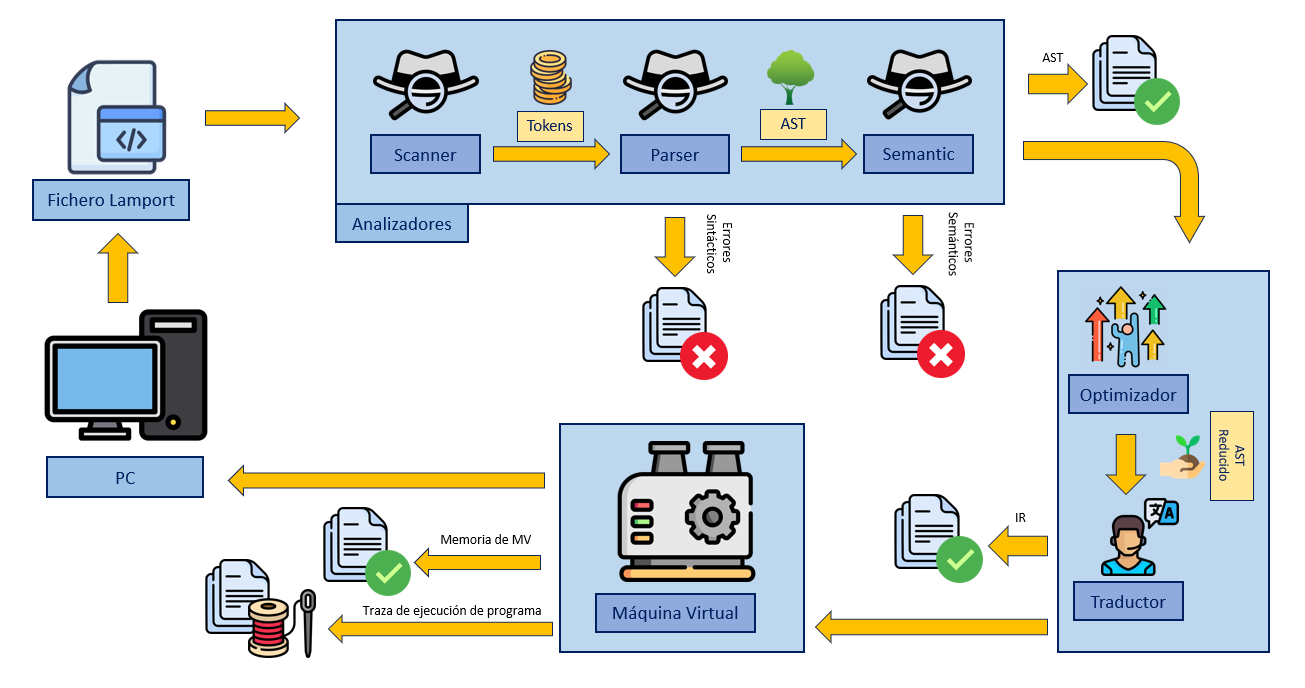
\includegraphics[width=\linewidth]{images/lmp/lmp_resume.png}
    \caption{Esquemático del intérprete de Lamport}
    \label{fig:lmpresume}
\end{figure}



\begin{itemize}
    \item \textbf{Lexer (~\ref{sec:implementacionLexer} ):} Implementa el analizador léxico con Flex. Es el primer módulo encargado de escanear el fichero, reconociendo todos los patrones y obteniendo los tokens.
    
    \item \textbf{Parser (~\ref{sec:implementacionParser} ):} Implementa el analizador sintáctico con Bison. Su función es analizar la secuencia de tokens proporcionada por el Lexer y construir una representación estructurada: un Árbol de Sintaxis Abstracta.
    
    \item \textbf{AST (~\ref{sec:implementacionAST} ):} Representa el Árbol de Sintaxis Abstracta. Es una representación gráfica estructurada del código fuente, que es creada a partir del análisis realizado por el Parser.
    
    \item \textbf{Semantic (~\ref{sec:implementacionSemantic} ):} Encargado del análisis semántico. Evalúa el AST para asegurarse de que el programa cumple con todas las reglas semánticas.
    
    \item \textbf{Error (~\ref{sec:implementacionError} ):} Gestiona y reporta errores encontrados en cualquier etapa de la interpretación, ya sea en el análisis léxico, sintáctico o semántico.
    
    \item \textbf{IR (~\ref{sec:implementacionError} ):} Representa la Representación Intermedia. Es una versión intermedia del código fuente que se utiliza para optimizaciones y para la generación final de código.
    
    \item \textbf{LVM (~\ref{sec:implementacionLVM} ):} Se refiere a la Máquina Virtual de Lamport. Este módulo ejecuta el código representado en IR, actuando como el intérprete final que produce los resultados deseados.
    
    \item \textbf{LMP\_Utils (~\ref{sec:implementacionLMPUtils} ):} Consiste en una serie de controladores que coordinan y facilitan la interacción entre los diferentes módulos del intérprete.
    
\end{itemize}

\section{Módulo de análisis léxico: ``Lexer''}\label{sec:implementacionLexer}
El ``Lexer'' es crucial para la interpretación del lenguaje Lamport, y se ha seleccionado Flex para su implementación por su eficacia y compatibilidad con las especificaciones del lenguaje. Este módulo convierte el código fuente en tokens que luego utiliza el analizador sintáctico para formar el Árbol de Sintaxis Abstracta (AST), actuando como un enlace entre el código y el análisis sintáctico.

\subsection{Diseño y Funcionalidad del Lexer}
El Lexer se desarrolla en un archivo llamado \texttt{lexer.l}, siguiendo la estructura estándar de Flex. Este archivo se divide en secciones clave:

\begin{itemize}
    \item \textbf{Cabeceras y Funciones}: Incluye las bibliotecas necesarias y define funciones auxiliares, facilitando la integración con otras partes del sistema, como el analizador sintáctico.
    \item \textbf{Patrones de Reconocimiento y Acciones Asociadas}: Aquí se establecen las expresiones regulares para identificar tokens del lenguaje Lamport y las acciones correspondientes, como devolver tokens y manejar comentarios y espacios en blanco.
    \item \textbf{Función Central \texttt{yylex()}}: Generada automáticamente por Flex, esta función es el motor del Lexer, encargándose de leer la entrada, identificar patrones y ejecutar acciones asociadas.
\end{itemize}

\subsection{Desafíos y Soluciones en la Implementación}
La interdependencia entre el Lexer y el Parser, especialmente en la definición y reconocimiento de tokens, representa un desafío significativo. Los tokens se definen en una cabecera generada por Bison, requiriendo coordinación entre Flex y Bison. Además, el manejo de cadenas en C plantea desafíos en la memoria dinámica, particularmente al procesar literales e identificadores.

\subsection{Generación del Lexer}
El contenido del fichero \texttt{lexer.l} es procesado por Flex para generar un archivo de código C funcional. Este proceso incluye el manejo detallado de tipos de tokens y cadenas, así como la configuración para el seguimiento preciso de errores por línea. La función \texttt{yylex()} actúa como el núcleo del analizador léxico, proporcionando una interfaz esencial con el analizador sintáctico.

Este enfoque integrado asegura que el Lexer no solo tokenice eficientemente el código fuente de Lamport, sino que también se coordine de manera efectiva con el proceso de análisis sintáctico, contribuyendo así al funcionamiento general del intérprete.
\subsection{Procesamiento de ``Hola Mundo'' utilizando el ``Lexer''}
Ya se dispone de la primera unidad operativa del intérprete, por ello, ya se puede realizar la primera interpretación del programa ``Hola Mundo'' (~\ref{fig:lamportHolaMundo} ). Habilitando un código que permita leer flujos de entrada, y pasando como argumento el fichero donde se encuentra el programa en Lamport, el resultado que muestra el analizador léxico es la siguiente lista:

\begin{figure}[h]
\begin{verbatim}
S_PROGRAM IDENT DELIM_PC
S_VAR IDENT DELIM_2P T_INTEGER DELIM_PC 

S_PROCEDURE IDENT PAR_IZDO IDENT DELIM_2P T_STRING PAR_DCHO 
B_BEGIN 
PRINT PAR_IZDO LITERAL DELIM_C IDENT DELIM_C LITERAL PAR_DCHO DELIM_PC
B_END

S_FUNCTION IDENT PAR_IZDO IDENT DELIM_2P T_INTEGER PAR_DCHO 
    DELIM_2P T_INTEGER DELIM_PC 
S_VAR IDENT DELIM_2P T_INTEGER OP_ASSIGN
    PAR_IZDO OP_MINUS L_INTEGER OP_SUM L_INTEGER PAR_DCHO OP_MULT L_INTEGER 
    OP_MINUS L_INTEGER DELIM_PC
B_BEGIN 
RETURN IDENT OP_SUM IDENT DELIM_PC 
B_END 

S_PROCESS IDENT DELIM_PC 
S_VAR IDENT DELIM_2P T_STRING OP_ASSIGN LITERAL DELIM_PC
S_VAR IDENT DELIM_2P T_INTEGER OP_ASSIGN L_INTEGER DELIM_PC
B_BEGIN 
IDENT PAR_IZDO IDENT PAR_DCHO DELIM_PC 
IDENT OP_ASSIGN IDENT PAR_IZDO IDENT PAR_DCHO DELIM_PC 
PRINT PAR_IZDO LITERAL DELIM_C IDENT PAR_DCHO DELIM_PC 
B_END
\end{verbatim}
\caption{Programa ``¡Hola Mundo!'' Lamport: Secuencia de Tokens.}
\label{fig:tokensHolaMundo}
\end{figure}

\section{Módulo de análisis sintáctico: ``Parser''}\label{sec:implementacionParser}
El analizador sintáctico para el lenguaje Lamport, construido con Bison, juega un papel crucial en la transformación de la secuencia de tokens (proporcionada por el Lexer) en estructuras sintácticas. Bison, conocido por su eficiencia con gramáticas \code{LALR(1)}, ayuda a materializar y procesar la gramática de Lamport.

\subsection{Diseño y Estructura del Parser}
El analizador sintáctico se estructura en el archivo \code{parser.y}, siguiendo las pautas de Bison. Sus componentes principales incluyen:

\begin{itemize}
    \item \textbf{Cabeceras y Funciones}: Incluyen archivos de cabecera y definen funciones utilizadas en el análisis sintáctico.
    \item \textbf{Declaración de Tokens}: Declara tokens provenientes del Lexer.
    \item \textbf{Estructuras para el AST}: Especifica estructuras para construir el Árbol de Sintaxis Abstracta durante el análisis.
    \item \textbf{Asociatividad de Operaciones}: Establece la precedencia de operadores para evitar ambigüedades.
    \item \textbf{Reglas de producción y Acciones semánticas}: Constituyen el núcleo del Parser, definiendo la agrupación de tokens en estructuras sintácticas y permitiendo construir el AST.
\end{itemize}

\subsection{Solucionando los problemas de ambigüedad de la gramática}
Ha llegado el momento de asegurar que los conflictos derivados de la definición ambigüa de la gramática (~\ref{subsubsec:gramaticaAmbiguaLamport} ) se resuelven e implementan de la manera más eficiente para la generación del analizador sintáctico en la práctica.


\noindent
Para generar el analizador sintáctico y además asegurar que no se producen conflictos, se utilizará la siguiente orden:
\begin{verbatim}
    bison --defines=include/lexer/token.h --output=src/parser/parser.c 
        src/parser/parser.y -Wcounterexamples
\end{verbatim}

La opción más notable en este comando es \code{-Wcounterexamples}. Esta opción instruye a Bison a mostrar ejemplos concretos de entrada cuando se detectan conflictos en la gramática. Es especialmente útil ya que no sólo informa de la existencia de un conflicto, sino que también proporciona una entrada específica que lo desencadena, facilitando así la tarea de identificar y corregir el problema en la gramática.

\newpage

\subsubsection{Expresiones}
Si se intenta generar la gramática de Lamport definida en ~\ref{sec:gramaticaLamport} directamente, ocurrirá lo siguiente:
\begin{figure}[h]
    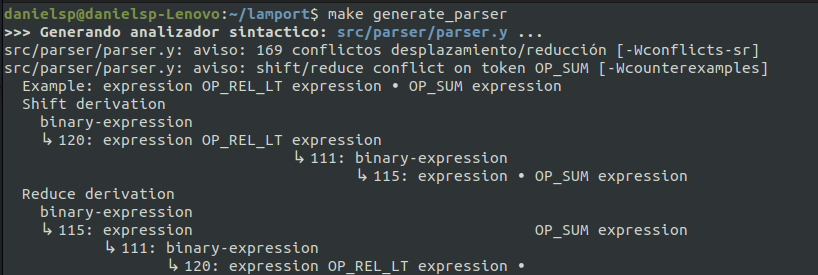
\includegraphics[width=\linewidth]{images/implementacion/parser/parser_conflicts.png}
    \caption{Conflictos de generación de parser por ambigüedad de gramática.}
    \label{fig:parser_conflictos}
\end{figure}

Se producen una inmensa cantidad de conflictos de tipo deslplazamiento/reducción (169 en total). En la captura se observa la indecisión de Bison para decantarse por una regla u otra con el ejemplo siguiente, donde se muestran dos caminos posibles para obtener la misma producción:

\begin{verbatim}
    expression OP_REL_LT expression * OP_SUM expression
\end{verbatim}



La solución para este problema en particular pasa por utilizar la precedencia de los operadores que ya se definió en la sección (~\ref{subsec:precOperadoresLamport} ). En Bison se puede indicar utilizando las directivas:

\begin{verbatim}
    %left <TOKEN>
    %right <TOKEN>
\end{verbatim}

\noindent
donde \code{\%left} y \code{\%right} especifican la asociatividad de las operaciones.



Ahora el resultado es este, donde ya podemos garantizar que $G$ es una gramática \code{LALR(1)}, que es lo que queríamos demostrar al generar la gramática con Bison:
\begin{figure}[h]
    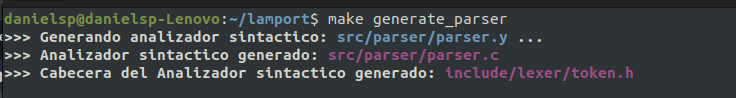
\includegraphics[width=\linewidth]{images/implementacion/parser/parser_success.png}
    \caption{Generación exitosa de la gramática de Lamport.}
    \label{fig:parser_success}
\end{figure}

\subsection{Estrategia de recuperación ante errores sintácticos}
Otro de los problemas a abordar ahora es qué hacer cuando el analizador sintáctico se encuentra con una estructura de tokens que no corresponde con ninguna de las previstas. Aquí hay dos formas posibles de implementar este mecanismo:

\begin{enumerate}
    \item Detectar un error sintáctico y detener inmediatamente el análisis mediante la directiva \code{YYABORT}. Esta acción provoca que, al identificar el primer error en el programa, este sea reconocido y gestionado adecuadamente. Acto seguido, el analizador sintáctico se detendrá, evitando el análisis del resto del fichero.
    
    \item Detectar un error sintáctico e intentar recuperarse, reanudando el análisis a partir de un token específico. En este enfoque, al encontrar un error, se gestiona y, posteriormente, se indica al analizador sintáctico un punto específico dentro de la secuencia de tokens restantes para que continúe con el análisis.
\end{enumerate}

Ambas estrategias son válidas y tienen sus méritos. Sin embargo, es esencial considerar la experiencia del usuario al decidir cuál implementar. La segunda opción, aunque es técnicamente más desafiante debido a la necesidad de identificar los puntos precisos para la recuperación, puede ofrecer una experiencia de usuario más amigable al proporcionar retroalimentación más detallada sobre múltiples errores en lugar de detenerse en el primero. Finalmente, se ha adoptado utilizar un esquema híbrido donde se implementa el primer caso para detección de patrones no esperados y el segundo para detección de errores sintácticos más precisos, como por ejemplo errores en la declaración de una variable.

\section{Árbol de Sintaxis Abstracto (AST)}\label{sec:implementacionAST}
Tras completar el análisis sintáctico, surge la necesidad de representar el programa de una manera que facilite su manipulación y análisis en etapas subsecuentes. En este contexto, se introduce el Árbol de Sintaxis Abstracta (AST, por sus siglas en inglés). Un AST proporciona una representación estructurada y jerárquica de la estructura lógica del código fuente, prescindiendo de muchos detalles superficiales presentes en el texto original. En esta sección, se abordará la construcción y características del AST y se profundizará en su relevancia para el entendimiento y procesamiento del programa Lamport.

\subsection{Nodos del AST}
Dentro de la representación de un Árbol de Sintaxis Abstracta (AST), los nodos desempeñan un papel fundamental. Cada nodo refleja una construcción o elemento del lenguaje de programación, y la estructura jerárquica del árbol establece las relaciones entre estos elementos. En esta subsección, se abordarán los diferentes tipos de nodos que componen el AST, sus características y cómo contribuyen a capturar la esencia semántica del programa Lamport.



En la implementación práctica del AST, los nodos se manejan mediante punteros. Esta elección se justifica por diversas razones. Primero, usar punteros permite una gestión dinámica de memoria, lo que facilita la creación, modificación y eliminación de nodos durante el análisis sintáctico. Además, el uso de punteros posibilita la conexión directa entre nodos para formar la estructura de árbol. Esta metodología también optimiza la eficiencia en términos de memoria y acceso, dado que se evita la duplicación de datos y se permite una referencia directa a la información del nodo.


Todos los nodos citados a continuación han sido definidos mediante un \code{struct}, que es una estructura de datos en C que permite agrupar múltiples variables de diferentes tipos bajo un mismo nombre. Estos \code{structs} proporcionan una manera organizada y coherente de representar información compleja. Así, cada nodo del AST puede contener múltiples campos relevantes para su tipo específico, tales como operadores, operandos, identificadores, entre otros. 


De hecho, la estructura subyacente en la mayoría de los nodos (exceptuando el nodo raíz o padre que representa al programa completo) se basa en el concepto de \textbf{lista enlazada}, una estructura de datos muy utilizada en el ámbito de la programación. Esta estructura se emplea con el objetivo de definir secuencias de nodos de manera eficiente, indicando desde cada nodo la posición del siguiente en la lista.


\noindent
Para cada nodo además se implementaron los siguientes grupos de funciones:

\begin{itemize}
    \item \code{struct node * create_node(...)} : Función encargada de reservar memoria e inicializar un nodo en particular teniendo en cuenta los parámetros que se le han pasado a la función.
    \item \code{void free_node(struct node *)} : Función encargada de liberar la memoria reservada para el nodo pasado como parámetro.
    \item \code{void print_node(struct node *, int depth)} : Función encargada de imprimir el contenido del nodo pasado como parámetro en un flujo de salida. El entero \code{depth} especifica la profundidad del nodo en el árbol, para así poder imprimirlo en el lugar donde corresponde.
\end{itemize}

\noindent
Y en definitiva, estos son los diferentes tipos de nodos considerados:

\begin{enumerate}
    \item \textbf{Nodo de Expresión (expression)}: 
    \begin{itemize}
        \item Almacena información sobre expresiones binarias, unarias, identificadores, literales y llamadas a funciones.
        \item Permite encadenar múltiples expresiones y manejar operaciones complejas.
    \end{itemize}

    \item \textbf{Nodo de Tipo de Dato (type)}:
    \begin{itemize}
        \item Define el tipo de dato (básico, array, especial) de una variable.
        \item Incluye información sobre subtipos y línea de definición.
    \end{itemize}

    \item \textbf{Nodo de Declaración de Variable (declaration)}:
    \begin{itemize}
        \item Contiene identificador, tipo de dato y expresión asignada a una variable.
        \item Permite declarar variables con o sin asignación inicial.
    \end{itemize}

    \item \textbf{Nodo de Sentencia (statement)}:
    \begin{itemize}
        \item Representa diferentes tipos de sentencias (asignación, bucles, if/else, etc.).
        \item Incluye la estructura y la lógica de control y ejecución del programa.
    \end{itemize}

    \item \textbf{Nodo de Parámetro de Subprograma (parameter)}:
    \begin{itemize}
        \item Define los parámetros de subprogramas (funciones y procedimientos).
        \item Incluye nombre, tipo de dato y posición de definición.
    \end{itemize}

    \item \textbf{Nodo de Subprograma (subprogram)}:
    \begin{itemize}
        \item Representa funciones y procedimientos con sus parámetros y cuerpo.
        \item Incluye información de retorno para funciones.
    \end{itemize}

    \item \textbf{Nodo de Proceso (process)}:
    \begin{itemize}
        \item Define procesos, incluyendo nombre, índice y cuerpo de ejecución.
        \item Soporta procesos estáticos vectorizados y maneja declaraciones y sentencias.
    \end{itemize}

    \item \textbf{Nodo de Programa (program)}:
    \begin{itemize}
        \item Nodo raíz del AST que encapsula toda la estructura del programa.
        \item Incluye subprogramas, declaraciones globales y procesos.
    \end{itemize}
\end{enumerate}


\subsection{Integración del AST en el analizador sintáctico}
La integración del AST en el analizador sintáctico generado por Bison se realiza mediante acciones semánticas en las reglas gramaticales. Estas acciones permiten la construcción automática del AST durante el análisis sintáctico. Se emplean directivas específicas (\code{\%union}, \code{\%type}) para definir los tipos de datos que devolverán las reglas gramaticales y asociarlos con las estructuras del AST.

Un enfoque crucial en esta etapa es la gestión de la memoria dinámica, asegurando la reserva y liberación adecuada de memoria para los nodos del AST. Esto incluye estrategias para el manejo eficiente de errores y la prevención de fugas de memoria.

\subsection{Procesamiento de ``Hola Mundo'' utilizando el ``Parser'' con AST}
Ahora ya se puede dar forma a nivel estructural y computacional del código Lamport, y es por ello que ahora que el procesamiento de ``Hola Mundo'' (~\ref{fig:lamportHolaMundo} ) arrojará como resultado el AST que se genere, puesto que el programa es sintácticamente correcto.

\begin{verbatim}
----> PROGRAMA LAMPORT DE NOMBRE: [HolaMundo]
================================================================

----> | DECLARACIONES DE PROGRAMA: [HolaMundo]
|-----> DECLARACION DE VARIABLE: [magico]
|       TIPO DE DATO:
|           TIPO: [integer]
|       VALOR DE INICIALIZACION:
|           <NONE>

================================================================

----> | SUBPROGRAMAS DE PROGRAMA: [HolaMundo]
|-----> NOMBRE DE SUBPROGRAMA: [SaludaUsuario] DE TIPO: [procedure]
|       TIPO DE DATO DE RETORNO:
|   ----> <NONE>
|       PARAMETROS DE SUBPROGRAMA:
|         NOMBRE DE PARAMETRO: [nombre]
|         TIPO DE DATO: [nombre]
|           TIPO: [string]

|       DECLARACIONES DE SUBPROGRAMA:
|-------> <NONE>
|       SENTENCIAS DE SUBPROGRAMA:
|-------> | SENTENCIA DE TIPO: [begin/end block]
|-----------> | SENTENCIA DE TIPO: [print statement]
|             | LISTADO DE EXPRESIONES A IMPRIMIR:
|                > EXPRESION DE TIPO: [literal string]
|                  VALOR DE LITERAL: ["Hola "]
|                > EXPRESION DE TIPO: [identifier]
|                  NOMBRE DE IDENTIFICADOR: [nombre]
|                > EXPRESION DE TIPO: [literal string]
|                  VALOR DE LITERAL: ["!"]



|-----> NOMBRE DE SUBPROGRAMA: [ObtieneNumero] DE TIPO: [function]
|       TIPO DE DATO DE RETORNO:
|         TIPO: [integer]
|       PARAMETROS DE SUBPROGRAMA:
|         NOMBRE DE PARAMETRO: [n]
|         TIPO DE DATO: [n]
|           TIPO: [integer]

|       DECLARACIONES DE SUBPROGRAMA:
|-------> DECLARACION DE VARIABLE: [constant]
|         TIPO DE DATO:
|             TIPO: [integer]
|         VALOR DE INICIALIZACION:
|            > EXPRESION DE TIPO: [binary operation]
|              SIMBOLO DE OPERACION: [-]
|              OPERANDO IZQUIERDO:
|                > EXPRESION DE TIPO: [binary operation]
|                  SIMBOLO DE OPERACION: [*]
|                  OPERANDO IZQUIERDO:
|                    > EXPRESION DE TIPO: [grouped expression]
|                      EXPRESION ENTRE ( )
|                        > EXPRESION DE TIPO: [binary operation]
|                          SIMBOLO DE OPERACION: [+]
|                          OPERANDO IZQUIERDO:
|                            > EXPRESION DE TIPO: [unary operation]
|                              SIMBOLO DE OPERACION: [-]
|                              OPERANDO IZQUIERDO:
|                                > EXPRESION DE TIPO: [literal integer]
|                                  VALOR DE LITERAL: [4]
|                          OPERANDO DERECHO:
|                            > EXPRESION DE TIPO: [literal integer]
|                              VALOR DE LITERAL: [6]
|                  OPERANDO DERECHO:
|                    > EXPRESION DE TIPO: [literal integer]
|                      VALOR DE LITERAL: [10]
|              OPERANDO DERECHO:
|                > EXPRESION DE TIPO: [literal integer]
|                  VALOR DE LITERAL: [2]

|       SENTENCIAS DE SUBPROGRAMA:
|-------> | SENTENCIA DE TIPO: [begin/end block]
|-----------> | SENTENCIA DE TIPO: [return statement]
|             | EXPRESION DE RETORNO:
|                > EXPRESION DE TIPO: [binary operation]
|                  SIMBOLO DE OPERACION: [+]
|                  OPERANDO IZQUIERDO:
|                    > EXPRESION DE TIPO: [identifier]
|                      NOMBRE DE IDENTIFICADOR: [constant]
|                  OPERANDO DERECHO:
|                    > EXPRESION DE TIPO: [identifier]
|                      NOMBRE DE IDENTIFICADOR: [n]



================================================================

----> | PROCESOS DEL PROGRAMA: [HolaMundo]
|-----> | NOMBRE DE PROCESO: [Main] DE TIPO: [individual process]

|-----> | DECLARACIONES DE PROCESO:
|---------> DECLARACION DE VARIABLE: [usuario]
|           TIPO DE DATO:
|               TIPO: [string]
|           VALOR DE INICIALIZACION:
|              > EXPRESION DE TIPO: [literal string]
|                VALOR DE LITERAL: ["Daniel"]

|---------> DECLARACION DE VARIABLE: [numero]
|           TIPO DE DATO:
|               TIPO: [integer]
|           VALOR DE INICIALIZACION:
|              > EXPRESION DE TIPO: [literal integer]
|                VALOR DE LITERAL: [23]


|-----> | SENTENCIAS DE PROCESO:
|---------> | SENTENCIA DE TIPO: [begin/end block]
|-------------> | SENTENCIA DE TIPO: [procedure invocation]
|               | INVOCACION DE PROCEDIMIENTO DE NOMBRE: [SaludaUsuario]
|               | LISTADO DE ARGUMENTOS DE INVOCACION DEL PROCEDIMIENTO:
|                  > EXPRESION DE TIPO: [identifier]
|                    NOMBRE DE IDENTIFICADOR: [usuario]

|-------------> | SENTENCIA DE TIPO: [assignment]
|               | ASIGNACION A VARIABLE: [magico]
|               | EXPRESION ASIGNADA A VARIABLE:
|                  > EXPRESION DE TIPO: [function invocation]
|                    INVOCACION DE FUNCION DE NOMBRE: [ObtieneNumero]
|                    LISTADO DE ARGUMENTOS DE INVOCACION DE FUNCION:
|                      > EXPRESION DE TIPO: [identifier]
|                        NOMBRE DE IDENTIFICADOR: [numero]

|-------------> | SENTENCIA DE TIPO: [print statement]
|               | LISTADO DE EXPRESIONES A IMPRIMIR:
|                  > EXPRESION DE TIPO: [literal string]
|                    VALOR DE LITERAL: ["El numero magico vale: "]
|                  > EXPRESION DE TIPO: [identifier]
|                    NOMBRE DE IDENTIFICADOR: [magico]
\end{verbatim}
\begin{figure}[hbtp]
\caption{Programa ``¡Hola Mundo!'' Lamport: Resultado de análisis sintáctico (AST).}
\label{fig:ASTHolaMundo}
\end{figure}

\section{Módulo de análisis semántico: ``Semantic''}\label{sec:implementacionSemantic}
El análisis semántico en el lenguaje Lamport verifica la coherencia y correctitud del código más allá de la gramática, enfocándose en las reglas de contexto y las relaciones semánticas. Este módulo es importante para asegurar que el código tenga un significado lógico y esté listo para la interpretación.

\subsection{La tabla de Símbolos}
La tabla de símbolos es un registro organizado de todas las entidades definidas en el código, como variables, constantes, funciones y procedimientos. Esta tabla almacena información crucial, incluyendo tipo, alcance y, en algunos casos, valores iniciales o información de memoria.

\subsubsection{Ámbito de variable (scope) y Tabla de Símbolos}
El ámbito de una variable, o su \textit{scope}, define su accesibilidad en el código, pudiendo ser global (accesible en todo el programa) o local (limitada a un bloque específico). Para manejar los ámbitos eficientemente, se utiliza una tabla hash en la tabla de símbolos. Esta estructura, que asocia claves (nombres de símbolos) con valores (información del símbolo), permite un acceso rápido y eficiente a los datos mediante funciones hash.

\subsubsection{Implementación de la tabla con una pila de tablas hash}
La gestión de los diferentes ámbitos se realiza a través de una pila de tablas hash. Al entrar en un nuevo ámbito, como un subprograma o proceso, se añade una tabla hash vacía a la cima de la pila, donde los símbolos definidos en ese ámbito se almacenarán. Al salir del ámbito, la tabla hash correspondiente se retira, eliminando los símbolos de ese ámbito específico. Esta estructura facilita la resolución de referencias a símbolos, siempre resolviendo al símbolo más cercano en términos de ámbito.

Para llevar a cabo esta tarea, se deben enfrentar varios desafíos. En primer lugar, es necesario identificar y gestionar los distintos ámbitos o ``scopes'' en los que un nombre puede estar definido. Como se ha visto en secciones anteriores, la estructura de una pila de tablas hash es útil en este aspecto. Cada ámbito tiene su propia tabla hash, y al buscar un nombre, se consulta primero la tabla del ámbito actual, avanzando hacia ámbitos más externos si es necesario.

\subsection{Resolución de nombres}
El análisis semántico comienza con la resolución de nombres, determinando a qué entidad del programa se refiere un nombre en un contexto dado. Esta fase es crucial para garantizar la coherencia y correcta ejecución del código, empleando la estructura de la pila de tablas hash para identificar correctamente los ámbitos y resolver las referencias a símbolos

El esquema general del algoritmo de resolución de nombres es el siguiente, aplicándolo desde el nodo raíz del AST (\code{program}):
\begin{enumerate}
    \item Al inicio del análisis:
    \begin{enumerate}
        \item Insertar el ``scope'' global en la pila.
    \end{enumerate}
    \item Si se trata de un bloque de declaraciones:
    \begin{enumerate}
        \item Comprobar si ya existe un símbolo en la tabla de símbolos para la variable actual a analizar.
        \begin{itemize}
            \item En caso afirmativo, se trata de un \textbf{error de redefinición de variable}.
            \item En otro caso, se crea el símbolo y se inserta en el ``scope''.
        \end{itemize}
        \item Continuar con el resto de variables hasta que no queden.
    \end{enumerate}
    \item Si se trata de un bloque de sentencias/expresiones:
    \begin{itemize}
        \item Aplicar resolución de nombres a cada sentencia o expresión hasta que no queden, buscando en todos los scopes las posibles referencias a símbolos que puedan haber.
        \begin{itemize}
            \item Si no se encuentra una referencia a un símbolo dentro de unas estructuras, se trata de un \textbf{error de uso de símbolo no declarado}, ya sea de variable, subprograma o proceso.
        \end{itemize}
    \end{itemize}
    \item Si se trata de un bloque de subprogramas:
    \begin{enumerate}
        \item Comprobar para el scope global y para el subprograma actual a analizar si ya existe un símbolo en la tabla de símbolos asociado a su identificador.
        \begin{itemize}
            \item En caso afirmativo, se tata de un \textbf{error de redefinición de subprograma}.
            \item En otro caso, se crea el símbolo y se inserta en el ``scope''.
        \end{itemize}
        \item Insertar un nuevo ``scope'' en la pila.
        \item Aplicar resolución de nombres a las declaraciones del subprograma.
        \item Aplicar resolución de nombres a las sentencias del subprograma.
        \item Retirar el ``scope'' actual de la pila.

        \item Continuar con el resto de subprogramas hasta que no queden.
    \end{enumerate}
    \item Si se trata de un bloque de procesos:
    \begin{enumerate}
        \item Comprobar para el scope global y para el proceso actual a analizar si ya existe un símbolo en la tabla de símbolos asociado a su identificador.
        \begin{itemize}
            \item En caso afirmativo, se tata de un \textbf{error de redefinición de proceso}.
            \item En otro caso, se crea el símbolo y se inserta en el ``scope''.
        \end{itemize}
        \item Insertar un nuevo ``scope'' en la pila.
        \item Aplicar resolución de nombres a las declaraciones del proceso.
        \item Aplicar resolución de nombres a las sentencias del proceso.
        \item Retirar el ``scope'' actual de la pila.

        \item Continuar con el resto de procesos hasta que no queden.
    \end{enumerate}
\end{enumerate}

\subsection{Comprobación de tipos}
Esta fase garantiza que las operaciones y asignaciones realizadas en el código fuente son coherentes desde el punto de vista de los tipos de datos involucrados. Así, se evita que, por ejemplo, se intente sumar un número entero con una cadena de texto o que se asigne un valor de tipo real a una variable que espera un valor booleano.



La comprobación de tipos no solo proporciona seguridad en la ejecución al detectar errores potenciales en una etapa temprana del proceso de compilación, sino que también contribuye a la claridad y robustez del código. Aquí es donde entra en juego la descripción semántica que se hizo del lenguaje Lamport en ~\ref{subsec:semanticaLamport}, porque se aplicará directamente en este apartado del analizador semántico.



Con respecto a la comprobación de tipos \textit{per se} no hay ninguna dificultad técnica. La forma de proceder es prácticamente idéntica a la del algoritmo de resolución de nombres, recorriendo el AST comprobando todos los nodos importantes:

\begin{enumerate}
    \item Si se trata de una expresión:
    \begin{itemize}
        \item Comprobar que se verifican todas las restricciones semánticas definidas en ~\ref{subsubsec:restriccionesSemanticas} y que refieren a expresiones.
        \item En caso contrario, se produce un \textbf{error de comprobación de tipos entre operandos de expresión}.
        \item En el caso de una expresión de llamada a función, se debe comprobar que el tipo de los argumentos pasados coincide con el de los parámetros que se definieron para la función, en el mismo orden en el que aparecen éstos.
    \end{itemize}
    \item Si se trata de una declaración de variable y además tiene un valor de inicio:
    \begin{itemize}
        \item Comprobar que el tipo de dato de la variable coincide con la evaluación del tipo de dato que emite la expresión de inicialización.
        \item En caso contrario, se produce un \textbf{error de asignación de tipos}.
    \end{itemize}
    \item Si se trata de un subprograma:
    \begin{itemize}
        \item Comprobar que se verifican todas las restricciones semánticas definidas en ~\ref{subsubsec:restriccionesSemanticas} y que refieren a subprogramas.
        \item En caso contrario, se produce un \textbf{error de comprobación de tipos}.
    \end{itemize}
    \item Si se trata de una sentencia:
    \begin{itemize}
        \item Si se está realizando una sentencia de asignación, mismo tratamiento que en el caso de inicialización de variables.
        \item En el caso de bucles while y estructuras if/else, la expresión de condición debe emitir el tipo \code{boolean}.
        \item En el caso de bucles for, las expresiones de inicio y fin deben emitir el tipo \code{integer}.
        \item En el caso de una llamada a procedimiento, se debe comprobar que el tipo de los argumentos pasados coincide con el de los parámetros que se definieron para el procedimiento, en el mismo orden en el que aparecen éstos.
        \item Todo lo anterior que no se verifique será un \textbf{error de comprobación de tipos ó de asignación}.
    \end{itemize}
\end{enumerate}

\subsection{Procesamiento de ``Hola Mundo'' utilizando el ``Semantic''}
Ahora ya se dispone de todos los analizadores posibles para un lenguaje de programación cualquiera, en particular para el lenguaje Lamport. Adaptando el código del intérprete ahora cuando se supere la fase del analizador sintáctico, se recorrerá el AST generado analizando semánticamente el programa. Primero se aplica resolución de nombres y posteriormente la comprobación de tipos. Si el procesamiento de ``Hola Mundo'' (~\ref{fig:lamportHolaMundo} ) se ha superado, se verá un mensaje de éxito en pantalla. En caso contrario se mostrarán todos los errores semánticos emitidos:



\noindent
Puesto que el programa es semánticamente correcto, el mensaje que se muestra es:
\begin{verbatim}
    ``RESOLUCIÓN DE NOMBRES Y COMPROBACIÓN DE TIPOS 
        REALIZADOS CON ÉXITO.''
\end{verbatim}

\section{Módulo de gestión de errores: ``Error''}\label{sec:implementacionError}
Para manejar errores en los análisis sintáctico y semántico, se ha desarrollado un módulo específico de gestión de errores. Se utiliza una estructura común \code{error} que registra el tipo de error (sintáctico o semántico), la línea del error, un mensaje descriptivo y un puntero al siguiente error. La estructura también incluye detalles adicionales sobre errores específicos, tanto sintácticos como semánticos.

Este módulo de errores se integra tanto en el análisis sintáctico como en el semántico, marcando errores en las reglas sintácticas y a lo largo de los algoritmos semánticos. El orden de aparición de los errores depende de la fase de análisis:

\begin{enumerate}
    \item Si no se supera el análisis sintáctico, se imprimen los errores sintácticos.
    \item Si se supera el análisis sintáctico pero no la resolución de nombres, se imprimen los errores semánticos relacionados.
    \item Si no se supera la comprobación de tipos, se imprimen los errores semánticos correspondientes.
\end{enumerate}


\section{Módulo de gestión de Representación Intermedia: ``IR''}\label{sec:implementacionIR}
La Representación Intermedia (IR) es una fase fundamental en la transformación y optimización del código fuente de Lamport. Este módulo actúa como un puente entre el análisis semántico y la traducción final o interpretación del código, optimizando las operaciones posteriores mediante una estructura común y coherente.

\subsection{Elección de Representación Intermedia}
La IR elegida para este proyecto se basa en registros, con un conjunto de instrucciones que detallan el manejo de estos registros. Esta estructura facilita la simulación del funcionamiento de un sistema concurrente y simplifica la representación del código.

\noindent
Una instrucción consta de los siguientes elementos:

\begin{itemize}
    \item \textbf{Código de instrucción}: Es un identificador que sirve para indicar a la posterior máquina virtual el tipo de instrucción que va a ejecutar.
    \item \textbf{Operando de destino}: Identificador que representa el lugar donde el resultado de la acción que realizará la entidad que ejecute la instrucción se almacenará.
    \item \textbf{Operando 1}: Identificador que representa al dato del primer operando de la instrucción.
    \item \textbf{Operando 2}: Identificador que representa al dato del segundo operando de la instrucción.
\end{itemize}

Los operandos son elementos que determinan las fuentes de datos o valores con los que se realizará la operación indicada por el código de instrucción. Estos pueden ser constantes, registros, direcciones de memoria, entre otros. La cantidad y el tipo de operandos pueden variar según la instrucción, y su correcta interpretación es crucial para el adecuado funcionamiento de la máquina virtual y la ejecución del programa. En esta representación intermedia, hay estos tipos de operandos:

\begin{itemize}
    \item \textbf{Identificación de un registro}: El operando apunta a un registro de la máquina virtual.
    \item \textbf{Identificación de un literal}: El operando apunta a un literal.
    \item \textbf{Identificación de una variable}: El operando apunta a una variable.
    \item \textbf{Identificación de una variable array}: El operando apunta a un elemento en concreto de una variable array.
    \item \textbf{Identificación de una etiqueta}: El operando apunta a la dirección de una etiqueta.
    \item \textbf{Identificación de un proceso/hebra}: El operando contiene el identificador del proceso.
    \item \textbf{Identificación de un salto directo}: El operando contiene la dirección de la siguiente instrucción a la que el proceso debe saltar. Tiene un comportamiento similar al de una etiqueta, pero sin especificar un nombre para la misma.
\end{itemize}

Finalmente, en este lenguaje de representación intermedia hay un total de \textbf{5 tipos de instrucciones diferentes}:

\begin{itemize}
    \item \textbf{1 destino y 2 operandos}: la instrucción a ejecutar necesita de dos operandos y el resultado se almacenará en un destino.
    \item \textbf{1 destino y 1 operando}: la instrucción a ejecutar necesita un operando y el resultado se almacena en un destino.
    \item \textbf{1 operando}: la instrucción a ejecutar necesita un operando, y no hay necesidad de almacenar el resultado de la acción.
    \item \textbf{0 destinos y 2 operandos}: la instrucción dispone de dos operandos pero no se almacena el resultado de la ejecución en un destino.
    \item \textbf{0 destinos y 0 operandos}: la instrucción sólo dispone de su código de instrucción, suficiente para su ejecución.
\end{itemize}

\subsection{Repertorio de instrucciones de IR}
A continuación se realiza un estudio detallado del repertorio de instrucciones definido para la representación intermedia del lenguaje Lamport.

\renewcommand{\arraystretch}{1.5}
\begin{longtable}{|c|c|c|c|c|}
\caption{Repertorio de instrucciones de Representación Intermedia.} \label{tab:instruccionesIR} \\
\hline
\textbf{CÓDIGO} & \textbf{DETALLES} & \textbf{OP. DEST.} & \textbf{OP. 1} & \textbf{OP. 2} \\
\hline
\endfirsthead

\multicolumn{5}{c}%
{{\bfseries \tablename\ \thetable{} -- continuación de la página anterior}} \\
\hline
\textbf{CÓDIGO} & \textbf{DETALLES} & \textbf{OP. DEST.} & \textbf{OP. 1} & \textbf{OP. 2} \\
\hline
\endhead

\hline \multicolumn{5}{|r|}{{Continúa en la siguiente página}} \\
\hline
\endfoot

\hline
\endlastfoot
\code{IR_LABEL} & ~\ref{subsubsec:IR_LABEL}  & NO & SÍ & NO \\
\hline
\code{IR_OP_LOAD} & ~\ref{subsubsec:IR_OP_LOAD}  & SÍ & SÍ & NO \\
\hline
\code{IR_OP_STORE} & ~\ref{subsubsec:IR_OP_STORE} & SÍ & SÍ & NO \\
\hline
\code{IR_OP_ADD_[I|F]} \footnote{Aquí y en el resto de instrucciones aritméticas, ``I'' denota que la instrucción involucra a operandos de tipo \textbf{entero}, mientras que ``F'' hace lo mismo con operandos de tipo \textbf{real}.} & ~\ref{subsubsec:IR_OP_ADD} & SÍ & SÍ & SÍ \\
\hline
\code{IR_OP_SUB_[I|F]} & ~\ref{subsubsec:IR_OP_SUB} & SÍ & SÍ & SÍ \\
\hline
\code{IR_OP_MULT_[I|F]} & ~\ref{subsubsec:IR_OP_MULT} & SÍ & SÍ & SÍ \\
\hline
\code{IR_OP_DIV_[I|F]} & ~\ref{subsubsec:IR_OP_DIV} & SÍ & SÍ & SÍ \\
\hline
\code{IR_OP_MOD_I} & ~\ref{subsubsec:IR_OP_MOD} & SÍ & SÍ & SÍ \\
\hline
\code{IR_OP_NEG_[I|F]} & ~\ref{subsubsec:IR_OP_NEG} & SÍ & SÍ & SÍ \\
\hline
\code{IR_OP_AND} & ~\ref{subsubsec:IR_OP_AND} & SÍ & SÍ & SÍ \\
\hline
\code{IR_OP_OR} & ~\ref{subsubsec:IR_OP_OR} & SÍ & SÍ & SÍ \\
\hline
\code{IR_OP_NOT} & ~\ref{subsubsec:IR_OP_NOT} & SÍ & SÍ & SÍ \\
\hline
\code{IR_OP_CMP_LT} & ~\ref{subsubsec:IR_OP_CMP_LT} & SÍ & SÍ & SÍ \\
\hline
\code{IR_OP_CMP_LTE} & ~\ref{subsubsec:IR_OP_CMP_LTE} & SÍ & SÍ & SÍ \\
\hline
\code{IR_OP_CMP_GT} & ~\ref{subsubsec:IR_OP_CMP_GT} & SÍ & SÍ & SÍ \\
\hline
\code{IR_OP_CMP_GTE} & ~\ref{subsubsec:IR_OP_CMP_GTE} & SÍ & SÍ & SÍ \\
\hline
\code{IR_OP_CMP_EQ} & ~\ref{subsubsec:IR_OP_CMP_EQ} & SÍ & SÍ & SÍ \\
\hline
\code{IR_OP_CMP_NEQ} & ~\ref{subsubsec:IR_OP_CMP_NEQ} & SÍ & SÍ & SÍ \\
\hline
\code{IR_OP_JMP} & ~\ref{subsubsec:IR_OP_JMP} & NO & SÍ & NO \\
\hline
\code{IR_OP_JMP_TRUE} & ~\ref{subsubsec:IR_OP_JMP_TRUE} & NO & SÍ & NO \\
\hline
\code{IR_OP_JMP_FALSE} & ~\ref{subsubsec:IR_OP_JMP_FALSE} & NO & SÍ & NO \\
\hline
\code{IR_OP_CALL} & ~\ref{subsubsec:IR_OP_CALL} & NO & SÍ & NO \\
\hline
\code{IR_OP_RET} & ~\ref{subsubsec:IR_OP_RET} & NO & SÍ & NO \\
\hline
\code{IR_OP_PUSH} & ~\ref{subsubsec:IR_OP_PUSH} & NO & SÍ & NO \\
\hline
\code{IR_OP_POP} & ~\ref{subsubsec:IR_OP_POP} & NO & SÍ & NO \\
\hline
\code{IR_OP_PRINT} & ~\ref{subsubsec:IR_OP_PRINT} & NO & SÍ & NO \\
\hline
\code{IR_END_PRINT} & ~\ref{subsubsec:IR_END_PRINT} & NO & NO & NO \\
\hline
\code{IR_START_PROGRAM} & ~\ref{subsubsec:IR_START_PROGRAM} & NO & NO & NO \\
\hline
\code{IR_END_PROGRAM} & ~\ref{subsubsec:IR_END_PROGRAM} & NO & NO & NO \\
\hline
\code{IR_START_PROCESS} & ~\ref{subsubsec:IR_START_PROCESS} & NO & SÍ & NO \\
\hline
\code{IR_START_DPROCESS} & ~\ref{subsubsec:IR_START_DPROCESS} & SÍ & SÍ & SÍ \\
\hline
\code{IR_END_PROCESS} & ~\ref{subsubsec:IR_END_PROCESS} & NO & SÍ & NO \\
\hline
\code{IR_WAIT_PROCESS} & ~\ref{subsubsec:IR_WAIT_PROCESS} & NO & SÍ & NO \\
\hline
\code{IR_SLEEP_PROCESS} & ~\ref{subsubsec:IR_SLEEP_PROCESS} & NO & SÍ & NO \\
\hline
\code{IR_OP_ATOMIC_BEGIN} & ~\ref{subsubsec:IR_OP_ATOMIC_BEGIN} & NO & NO & NO \\
\hline
\code{IR_OP_ATOMIC_END} & ~\ref{subsubsec:IR_OP_ATOMIC_END} & NO & NO & NO \\
\hline
\code{IR_OP_SEM_WAIT} & ~\ref{subsubsec:IR_OP_SEM_WAIT} & NO & SÍ & NO \\
\hline
\code{IR_OP_SEM_SIGNAL} & ~\ref{subsubsec:IR_OP_SEM_SIGNAL} & NO & SÍ & NO \\
\hline
\code{IR_START_INIT_GLOBAL_VAR} & ~\ref{subsubsec:IR_START_INIT_GLOBAL_VAR} & NO & NO & NO \\
\hline
\code{IR_END_GLOBAL_VAR} & ~\ref{subsubsec:IR_END_INIT_GLOBAL_VAR} & NO & NO & NO \\
\end{longtable}
\renewcommand{\arraystretch}{1.0}

\subsubsection{Instrucción IR\_LABEL}\label{subsubsec:IR_LABEL}
\noindent
\textbf{Funcionalidad:} Representa a una etiqueta

\noindent
\textbf{Argumentos:} La estructura de la instrucción es la siguiente:
\begin{verbatim}
IR_LABEL <operando1>
\end{verbatim}
\begin{itemize}
    \item <\code{operando1}>: Etiqueta que delimita una sección.
\end{itemize}

\noindent
\textbf{Ejecución de la instrucción:}


\noindent
Se incrementa el contador de programa y se sigue el flujo de ejecución normal.


\noindent
\textbf{Ejemplo de uso:}
\begin{verbatim}
IR_LABEL etq1
\end{verbatim}

\subsubsection{Instrucción IR\_OP\_LOAD}\label{subsubsec:IR_OP_LOAD}
\noindent
\textbf{Funcionalidad:} Carga un valor de una variable en un registro.

\noindent
\textbf{Argumentos:} La estructura de la instrucción es la siguiente:
\begin{verbatim}
IR_OP_LOAD <registro_destino> <operando1>
\end{verbatim}
\begin{itemize}
    \item <\code{registro_destino}>: registro donde se almacenará el valor de la variable.
    \item <\code{operando1}>: Es una \code{variable}. Su valor se cargará en el registro de destino.
\end{itemize}

\noindent
\textbf{Ejecución de la instrucción:}
\noindent
Se realizan los siguientes pasos para la ejecución de la instrucción:

\begin{enumerate}
    \item El valor de <\code{operando1}> se carga en <\code{registro_destino}>.
\end{enumerate}

\noindent
\textbf{Ejemplo de uso:}
\noindent
Suponiendo que \code{y} es una variable:

\begin{verbatim}
IR_OP_LOAD R1, y
\end{verbatim}

\noindent
\textbf{Comentarios adicionales:}

La representación a nivel de código de esta instrucción realmente contendrá en el operando un entero apuntador a una tabla de variables indexada donde se encuentra el nombre de dicha variable \texttt{y}.

\subsubsection{Instrucción IR\_OP\_STORE}\label{subsubsec:IR_OP_STORE}
\noindent
\textbf{Funcionalidad:} Almacena el valor de un registro en una variable.

\noindent
\textbf{Argumentos:} La estructura de la instrucción es la siguiente:

\begin{verbatim}
IR_OP_STORE <registro_fuente> <operando1>
\end{verbatim}
\begin{itemize}
    \item <\code{registro_fuente}>: registro del cual se tomará el valor para almacenarlo en la variable.
    \item <\code{operando1}>: Es una \code{variable}. Se almacenará el valor del registro fuente en esta variable.
\end{itemize}

\noindent
\textbf{Ejecución de la instrucción:}
\noindent
Se realizan los siguientes pasos para la ejecución de la instrucción:

\begin{enumerate}
    \item El valor de <\code{registro_fuente}> se almacena en <\code{operando1}>.
\end{enumerate}

\noindent
\textbf{Ejemplo de uso:}
\noindent
Suponiendo que \code{z} es una variable:

\begin{verbatim}
IR_OP_STORE R2, z
\end{verbatim}

\noindent
\textbf{Comentarios adicionales:}

La representación a nivel de código de esta instrucción realmente contendrá en el operando un entero apuntador a una tabla de variables indexada donde se encuentra el nombre de dicha variable \texttt{z}.

\subsubsection{Instrucción IR\_OP\_ADD\_[I|F]}\label{subsubsec:IR_OP_ADD}
\noindent
\textbf{Funcionalidad:} Suma dos operandos y almacena el resultado en un registro.

\noindent
\textbf{Argumentos:} La estructura de la instrucción es la siguiente:
\begin{verbatim}
IR_OP_ADD_[I|F] <registro_destino> <operando1> <operando2>
\end{verbatim}
\begin{itemize}
    \item <\code{registro_destino}>: registro donde se almacenará el resultado de la suma.
    \item <\code{operando1}, \code{operando2}>: Operandos a sumar.
\end{itemize}

\noindent
\textbf{Ejecución de la instrucción:}


\noindent
El valor de <\code{operando1}> se suma al valor de <\code{operando2}>, y el resultado se almacena en <\code{registro_destino}>.


\noindent
\textbf{Ejemplo de uso:}
\begin{verbatim}
IR_OP_ADD_I R1, R2, R3
IR_OP_ADD_F R2, R3, R4
\end{verbatim}

\subsubsection{Instrucción IR\_OP\_SUB\_[I|F]}\label{subsubsec:IR_OP_SUB}
\noindent
\textbf{Funcionalidad:} Resta el segundo operando al primero y almacena el resultado en un registro.

\noindent
\textbf{Argumentos:} La estructura de la instrucción es la siguiente:
\begin{verbatim}
IR_OP_SUB_[I|F] <registro_destino> <operando1> <operando2>
\end{verbatim}
\begin{itemize}
    \item <\code{registro_destino}>: registro donde se almacenará el resultado de la resta.
    \item <\code{operando1}, \code{operando2}>: Operandos involucrados en la resta.
\end{itemize}

\noindent
\textbf{Ejecución de la instrucción:}
\vspace{0.3cm}

\noindent
El valor de <\code{operando2}> se resta del valor de <\code{operando1}>, y el resultado se almacena en <\code{registro_destino}>.
\vspace{0.3cm}

\noindent
\textbf{Ejemplo de uso:}
\begin{verbatim}
IR_OP_SUB_F R1, R2, R3
\end{verbatim}

\subsubsection{Instrucción IR\_OP\_MULT\_[I|F]}\label{subsubsec:IR_OP_MULT}
\noindent
\textbf{Funcionalidad:} Multiplica dos operandos y almacena el resultado en un registro.

\noindent
\textbf{Argumentos:} La estructura de la instrucción es la siguiente:
\begin{verbatim}
IR_OP_MULT_[I|F] <registro_destino> <operando1> <operando2>
\end{verbatim}
\begin{itemize}
    \item <\code{registro_destino}>: registro donde se almacenará el resultado de la multiplicación.
    \item <\code{operando1}, \code{operando2}>: Operandos a multiplicar.
\end{itemize}

\noindent
\textbf{Ejecución de la instrucción:}
\vspace{0.3cm}

\noindent
El valor de <\code{operando1}> se multiplica por el valor de <\code{operando2}>, y el resultado se almacena en <\code{registro_destino}>.
\vspace{0.3cm}

\noindent
\textbf{Ejemplo de uso:}
\begin{verbatim}
IR_OP_MULT_I R1, R2, R3
\end{verbatim}

\subsubsection{Instrucción IR\_OP\_DIV\_[I|F]}\label{subsubsec:IR_OP_DIV}
\noindent
\textbf{Funcionalidad:} Divide el primer operando entre el segundo y almacena el resultado en un registro.

\noindent
\textbf{Argumentos:} La estructura de la instrucción es la siguiente:
\begin{verbatim}
IR_OP_DIV_[I|F] <registro_destino> <operando1> <operando2>
\end{verbatim}
\begin{itemize}
    \item <\code{registro_destino}>: registro donde se almacenará el resultado de la división.
    \item <\code{operando1}, \code{operando2}>: Operandos involucrados en la división.
\end{itemize}

\noindent
\textbf{Ejecución de la instrucción:}
\vspace{0.3cm}

\noindent
El valor de <\code{operando1}> se divide entre el valor de <\code{operando2}>, y el resultado se almacena en <\code{registro_destino}>.
\vspace{0.3cm}

\noindent
\textbf{Ejemplo de uso:}
\begin{verbatim}
IR_OP_DIV_F R1, R2, R3
\end{verbatim}

\subsubsection{Instrucción IR\_OP\_MOD\_I}\label{subsubsec:IR_OP_MOD}
\noindent
\textbf{Funcionalidad:} Calcula el residuo de la división del primer operando entre el segundo y almacena el resultado en un registro.

\noindent
\textbf{Argumentos:} La estructura de la instrucción es la siguiente:
\begin{verbatim}
IR_OP_MOD_I <registro_destino> <operando1> <operando2>
\end{verbatim}
\begin{itemize}
    \item <\code{registro_destino}>: registro donde se almacenará el resultado del cálculo del residuo.
    \item <\code{operando1}, \code{operando2}>: Operandos involucrados en el cálculo del residuo.
\end{itemize}

\noindent
\textbf{Ejecución de la instrucción:}
\vspace{0.3cm}

\noindent
El residuo de la división del valor de <\code{operando1}> entre el valor de <\code{operando2}> se calcula, y el resultado se almacena en <\code{registro_destino}>.
\vspace{0.3cm}

\noindent
\textbf{Ejemplo de uso:}
\begin{verbatim}
IR_OP_MOD_I R1, R2, R3
\end{verbatim}

\subsubsection{Instrucción IR\_OP\_NEG\_[I|F]}\label{subsubsec:IR_OP_NEG}
\noindent
\textbf{Funcionalidad:} Realiza la negación aritmética del operando y almacena el resultado en un registro.

\noindent
\textbf{Argumentos:} La estructura de la instrucción es la siguiente:
\begin{verbatim}
IR_OP_NEG_[I|F] <registro_destino> <operando1>
\end{verbatim}
\begin{itemize}
    \item <\code{registro_destino}>: registro donde se almacenará el resultado de la negación.
    \item <\code{operando1}>: operando a negar.
\end{itemize}

\noindent
\textbf{Ejecución de la instrucción:}
\vspace{0.3cm}

\noindent
Se niega el valor de <\code{operando1}> y el resultado se almacena en \\
<\code{registro_destino}>.
\vspace{0.3cm}

\noindent
\textbf{Ejemplo de uso:}
\begin{verbatim}
IR_OP_NEG_I R0, R1
\end{verbatim}

\subsubsection{Instrucción IR\_OP\_AND}\label{subsubsec:IR_OP_AND}
\noindent
\textbf{Funcionalidad:} Realiza la conjunción lógica entre dos operandos y almacena el resultado en un registro.

\noindent
\textbf{Argumentos:} La estructura de la instrucción es la siguiente:
\begin{verbatim}
IR_OP_AND <registro_destino> <operando1> <operando2>
\end{verbatim}
\begin{itemize}
    \item <\code{registro_destino}>: registro donde se almacenará el resultado de la conjunción lógica.
    \item <\code{operando1}, \code{operando2}>: operandos de la conjunción lógica.
\end{itemize}

\noindent
\textbf{Ejecución de la instrucción:}
\vspace{0.3cm}

\noindent
Se realiza AND lógico entre los valores de <\code{operando1}> y <\code{operando2}> y el resultado se almacena en <\code{registro_destino}>.
\vspace{0.3cm}

\noindent
\textbf{Ejemplo de uso:}
\begin{verbatim}
IR_OP_AND R0, R1, $true
\end{verbatim}

\subsubsection{Instrucción IR\_OP\_OR}\label{subsubsec:IR_OP_OR}
\noindent
\textbf{Funcionalidad:} Realiza la disyunción lógica entre dos operandos y almacena el resultado en un registro.

\noindent
\textbf{Argumentos:} La estructura de la instrucción es la siguiente:
\begin{verbatim}
IR_OP_OR <registro_destino> <operando1> <operando2>
\end{verbatim}
\begin{itemize}
    \item <\code{registro_destino}>: registro donde se almacenará el resultado de la disyunción lógica.
    \item <\code{operando1}, \code{operando2}>: operandos de la disyunción lógica.
\end{itemize}

\noindent
\textbf{Ejecución de la instrucción:}
\vspace{0.3cm}

\noindent
Se realiza OR lógico entre los valores de <\code{operando1}> y <\code{operando2}> y el resultado se almacena en <\code{registro_destino}>.
\vspace{0.3cm}

\noindent
\textbf{Ejemplo de uso:}
\begin{verbatim}
IR_OP_OR R0, R1, R2
\end{verbatim}

\subsubsection{Instrucción IR\_OP\_NOT}\label{subsubsec:IR_OP_NOT}
\noindent
\textbf{Funcionalidad:} Realiza la negación lógica de un operando y almacena el resultado en un registro.

\noindent
\textbf{Argumentos:} La estructura de la instrucción es la siguiente:
\begin{verbatim}
IR_OP_NOT <registro_destino> <operando1>
\end{verbatim}
\begin{itemize}
    \item <\code{registro_destino}>: registro donde se almacenará el resultado de la operación lógica.
    \item <\code{operando1}>: operando de negación lógica. Puede ser: registro, literal.
\end{itemize}

\noindent
\textbf{Ejecución de la instrucción:}
\vspace{0.3cm}

\noindent
Se realiza NOT lógico de <\code{operando1}> y el resultado se almacena en <\code{registro_destino}>.
\vspace{0.3cm}

\noindent
\textbf{Ejemplo de uso:}
\begin{verbatim}
IR_OP_NOT R0, R1
\end{verbatim}


\subsubsection{Instrucción IR\_OP\_CMP\_LT}\label{subsubsec:IR_OP_CMP_LT}
\noindent
\textbf{Funcionalidad:} Compara si un operando es menor que otro y almacena el resultado de la comparación en un registro. El resultado será TRUE o FALSE.

\noindent
\textbf{Argumentos:} La estructura de la instrucción es la siguiente:
\begin{verbatim}
IR_OP_CMP_LT <registro_destino> <operando1> <operando2>
\end{verbatim}
\begin{itemize}
    \item <\code{registro_destino}>: registro donde se almacenará el resultado de la operación de comparación.
    \item <\code{operando1}> y <\code{operando2}>: operandos de comparación. Pueden ser: registro, literal.
\end{itemize}

\noindent
\textbf{Ejecución de la instrucción:}
\vspace{0.3cm}

\noindent
Se compara si <\code{operando1}> es menor que <\code{operando2}> y el resultado se almacena en <\code{registro_destino}>.
\vspace{0.3cm}

\noindent
\textbf{Ejemplo de uso:}
\begin{verbatim}
IR_OP_CMP_LT R0, R1, $5
\end{verbatim}

\subsubsection{Instrucción IR\_OP\_CMP\_LTE}\label{subsubsec:IR_OP_CMP_LTE}
\noindent
\textbf{Funcionalidad:} Compara si un operando es menor o igual que otro y almacena el resultado de la comparación en un registro. El resultado será TRUE o FALSE.

\noindent
\textbf{Argumentos:} La estructura de la instrucción es la siguiente:
\begin{verbatim}
IR_OP_CMP_LTE <registro_destino> <operando1> <operando2>
\end{verbatim}
\begin{itemize}
    \item <\code{registro_destino}>: registro donde se almacenará el resultado de la operación de comparación.
    \item <\code{operando1}> y <\code{operando2}>: operandos de comparación. Pueden ser: registro, literal.
\end{itemize}

\noindent
\textbf{Ejecución de la instrucción:}
\vspace{0.3cm}

\noindent
Se compara si <\code{operando1}> es menor o igual que <\code{operando2}> y el resultado se almacena en <\code{registro_destino}>.
\vspace{0.3cm}

\noindent
\textbf{Ejemplo de uso:}
\begin{verbatim}
IR_OP_CMP_LTE R0, R1, $5
\end{verbatim}

\subsubsection{Instrucción IR\_OP\_CMP\_GT}\label{subsubsec:IR_OP_CMP_GT}
\noindent
\textbf{Funcionalidad:} Compara si un operando es mayor que otro y almacena el resultado de la comparación en un registro. El resultado será TRUE o FALSE.

\noindent
\textbf{Argumentos:} La estructura de la instrucción es la siguiente:
\begin{verbatim}
IR_OP_CMP_GT <registro_destino> <operando1> <operando2>
\end{verbatim}
\begin{itemize}
    \item <\code{registro_destino}>: registro donde se almacenará el resultado de la operación de comparación.
    \item <\code{operando1}> y <\code{operando2}>: operandos de comparación. Pueden ser: registro, literal.
\end{itemize}

\noindent
\textbf{Ejecución de la instrucción:}
\vspace{0.3cm}

\noindent
Se compara si <\code{operando1}> es mayor que <\code{operando2}> y el resultado se almacena en <\code{registro_destino}>.
\vspace{0.3cm}

\noindent
\textbf{Ejemplo de uso:}
\begin{verbatim}
IR_OP_CMP_GT R0, R1, $5
\end{verbatim}

\subsubsection{Instrucción IR\_OP\_CMP\_GTE}\label{subsubsec:IR_OP_CMP_GTE}
\noindent
\textbf{Funcionalidad:} Compara si un operando es mayor o igual que otro y almacena el resultado de la comparación en un registro. El resultado será TRUE o FALSE.

\noindent
\textbf{Argumentos:} La estructura de la instrucción es la siguiente:
\begin{verbatim}
IR_OP_CMP_GTE <registro_destino> <operando1> <operando2>
\end{verbatim}
\begin{itemize}
    \item <\code{registro_destino}>: registro donde se almacenará el resultado de la operación de comparación.
    \item <\code{operando1}> y <\code{operando2}>: operandos de comparación. Pueden ser: registro, literal.
\end{itemize}

\noindent
\textbf{Ejecución de la instrucción:}
\vspace{0.3cm}

\noindent
Se compara si <\code{operando1}> es mayor o igual que <\code{operando2}> y el resultado se almacena en <\code{registro_destino}>.
\vspace{0.3cm}

\noindent
\textbf{Ejemplo de uso:}
\begin{verbatim}
IR_OP_CMP_GTE R0, R1, $5
\end{verbatim}


\subsubsection{Instrucción IR\_OP\_CMP\_EQ}\label{subsubsec:IR_OP_CMP_EQ}
\noindent
\textbf{Funcionalidad:} Compara si un operando es igual que otro y almacena el resultado de la comparación en un registro. El resultado será TRUE o FALSE.

\noindent
\textbf{Argumentos:} La estructura de la instrucción es la siguiente:
\begin{verbatim}
IR_OP_CMP_EQ <registro_destino> <operando1> <operando2>
\end{verbatim}
\begin{itemize}
    \item <\code{registro_destino}>: registro donde se almacenará el resultado de la operación de comparación.
    \item <\code{operando1}> y <\code{operando2}>: operandos de comparación. Pueden ser: registro, literal.
\end{itemize}

\noindent
\textbf{Ejecución de la instrucción:}
\vspace{0.3cm}

\noindent
Se compara si <\code{operando1}> es igual que <\code{operando2}> y el resultado se almacena en <\code{registro_destino}>.
\vspace{0.3cm}

\noindent
\textbf{Ejemplo de uso:}
\begin{verbatim}
IR_OP_CMP_EQ R0, R1, $5
\end{verbatim}

\subsubsection{Instrucción IR\_OP\_CMP\_NEQ}\label{subsubsec:IR_OP_CMP_NEQ}
\noindent
\textbf{Funcionalidad:} Compara si un operando es distinto que otro y almacena el resultado de la comparación en un registro. El resultado será TRUE o FALSE.

\noindent
\textbf{Argumentos:} La estructura de la instrucción es la siguiente:
\begin{verbatim}
IR_OP_CMP_NEQ <registro_destino> <operando1> <operando2>
\end{verbatim}
\begin{itemize}
    \item <\code{registro_destino}>: registro donde se almacenará el resultado de la operación de comparación.
    \item <\code{operando1}> y <\code{operando2}>: operandos de comparación. Pueden ser: registro, literal.
\end{itemize}

\noindent
\textbf{Ejecución de la instrucción:}
\vspace{0.3cm}

\noindent
Se compara si <\code{operando1}> es distinto que <\code{operando2}> y el resultado se almacena en <\code{registro_destino}>.
\vspace{0.3cm}

\noindent
\textbf{Ejemplo de uso:}
\begin{verbatim}
IR_OP_CMP_NEQ R0, R1, $5
\end{verbatim}

\subsubsection{Instrucción IR\_OP\_JMP}\label{subsubsec:IR_OP_JMP}
\noindent
\textbf{Funcionalidad:} Realiza un salto incondicional a la etiqueta especificada.

\noindent
\textbf{Argumentos:}
\begin{verbatim}
IR_OP_JMP <operando1>
\end{verbatim}
\begin{itemize}
    \item <\code{operando1}>: operando de salto. Es una \textit{etiqueta} que indica la entrada de un bloque de instrucciones.
\end{itemize}

\noindent
\textbf{Ejecución de la instrucción:}
\vspace{0.3cm}

\noindent
La ejecución se desplaza inmediatamente a la instrucción marcada por <\code{operando1}>.
\vspace{0.3cm}

\noindent
\textbf{Ejemplo de uso:}
\begin{verbatim}
IR_OP_JMP etq1
\end{verbatim}

\subsubsection{Instrucción IR\_OP\_JMP\_TRUE}\label{subsubsec:IR_OP_JMP_TRUE}
\noindent
\textbf{Funcionalidad:} Realiza un salto condicional a la etiqueta especificada si el valor de un registro es verdadero.

\noindent
\textbf{Argumentos:}
\begin{verbatim}
IR_OP_JMP_TRUE <operando1> <operando2>
\end{verbatim}
\begin{itemize}
    \item <\code{operando1}>: operando que contiene valor a evaluar (bool). Es un \textit{registro}.
    \item <\code{operando2}>: operando de salto. Es una \textit{etiqueta} que indica la entrada de un bloque de instrucciones.
\end{itemize}

\noindent
\textbf{Ejecución de la instrucción:}
\vspace{0.3cm}

\noindent
La ejecución se desplaza a la instrucción marcada por la etiqueta en <\code{operando2}> sólo si la evaluación del valor del registro en <\code{operando1}> es verdadero.
\vspace{0.3cm}

\noindent
\textbf{Ejemplo de uso:}
\begin{verbatim}
IR_OP_JMP_TRUE R0, etq2
\end{verbatim}

\subsubsection{Instrucción IR\_OP\_JMP\_FALSE}\label{subsubsec:IR_OP_JMP_FALSE}
\noindent
\textbf{Funcionalidad:} Realiza un salto condicional a la etiqueta especificada si el valor de un registro es falso.

\noindent
\textbf{Argumentos:}
\begin{verbatim}
IR_OP_JMP_FALSE <operando1> <operando2>
\end{verbatim}
\begin{itemize}
    \item <\code{operando1}>: operando que contiene valor a evaluar (bool). Es un \textit{registro}.
    \item <\code{operando2}>: operando de salto. Es una \textit{etiqueta} que indica la entrada de un bloque de instrucciones.
\end{itemize}

\noindent
\textbf{Ejecución de la instrucción:}
\vspace{0.3cm}

\noindent
La ejecución se desplaza a la instrucción marcada por la etiqueta en <\code{operando2}> sólo si la evaluación del valor del registro en <\code{operando1}> es falso.
\vspace{0.3cm}

\noindent
\textbf{Ejemplo de uso:}
\begin{verbatim}
IR_OP_JMP_FALSE R0, etq2
\end{verbatim}

\subsubsection{Instrucción IR\_OP\_CALL}\label{subsubsec:IR_OP_CALL}
\noindent
\textbf{Funcionalidad:} Realiza una llamada a un subprograma.

\noindent
\textbf{Argumentos:}
\begin{verbatim}
IR_OP_CALL <operando1>
\end{verbatim}
\begin{itemize}
    \item <\code{operando1}>: operando que indica el inicio de subprograma. Es una \textit{etiqueta}.
\end{itemize}

\noindent
\textbf{Ejecución de la instrucción:}
\vspace{0.3cm}

\noindent
Se guardan el contexto actual (dirección de retorno, registros,...) y la ejecución se desplaza al inicio del subprograma, indicado por el <\code{operando1}>.
\vspace{0.3cm}

\noindent
\textbf{Ejemplo de uso:}
\begin{verbatim}
IR_OP_CALL subprog_etq
\end{verbatim}

\subsubsection{Instrucción IR\_OP\_RET}\label{subsubsec:IR_OP_RET}
\noindent
\textbf{Funcionalidad:} Realiza un retorno de un subprograma.

\noindent
\textbf{Argumentos:}
\begin{verbatim}
IR_OP_RET
\end{verbatim}

\noindent
\textbf{Ejecución de la instrucción:}
\vspace{0.3cm}

\noindent
Se restaura el contexto guardado con anterioridad producido por una instrucción \texttt{IR\_OP\_CALL} y se desplaza la ejecución al punto justo después de la instrucción \texttt{IR\_OP\_CALL} realizada.
\vspace{0.3cm}

\noindent
\textbf{Ejemplo de uso:}
\begin{verbatim}
IR_OP_RET
\end{verbatim}


\subsubsection{Instrucción IR\_OP\_PUSH}\label{subsubsec:IR_OP_PUSH}
\noindent
\textbf{Funcionalidad:} Empuja un valor desde un registro específico a la pila de ejecución.

\noindent
\textbf{Argumentos:}
\begin{verbatim}
IR_OP_PUSH <operando1>
\end{verbatim}
\begin{itemize}
    \item <\code{operando1}>: operando que indica el valor. Es un \textit{registro}.
\end{itemize}

\noindent
\textbf{Ejecución de la instrucción:}
\vspace{0.3cm}

\noindent
Se leen el valor actual del registro especificado y se empuja este valor al tope de la pila de ejecución.
\vspace{0.3cm}

\noindent
\textbf{Ejemplo de uso:}
\begin{verbatim}
IR_OP_PUSH R1
\end{verbatim}

\subsubsection{Instrucción IR\_OP\_POP}\label{subsubsec:IR_OP_POP}
\noindent
\textbf{Funcionalidad:} Desapila el valor del tope de la pila de ejecución y lo almacena en un registro específico.

\noindent
\textbf{Argumentos:}
\begin{verbatim}
IR_OP_POP <operando1>
\end{verbatim}
\begin{itemize}
    \item <\code{operando1}>: operando que indica el lugar de almacenamiento. Es un \textit{registro}.
\end{itemize}

\noindent
\textbf{Ejecución de la instrucción:}
\vspace{0.3cm}

\noindent
Se desapila el valor del tope de la pila de ejecución y se almacena este valor en el registro especificado.
\vspace{0.3cm}

\noindent
\textbf{Ejemplo de uso:}
\begin{verbatim}
IR_OP_POP R1
\end{verbatim}

\subsubsection{Instrucción IR\_OP\_PRINT}\label{subsubsec:IR_OP_PRINT}
\noindent
\textbf{Funcionalidad:} Imprime el valor de un registro o literal en la salida estándar.

\noindent
\textbf{Argumentos:}
\begin{verbatim}
IR_OP_PRINT <operando1>
\end{verbatim}
\begin{itemize}
    \item <\code{operando1}>: Operando de impresión con el valor que se desea imprimir. Es un \textit{registro} o \textit{literal}.
\end{itemize}

\noindent
\textbf{Ejecución de la instrucción:}
\vspace{0.3cm}

\noindent
Se imprime el valor de <\code{operando1}>.
\vspace{0.3cm}

\noindent
\textbf{Ejemplo de uso:}
\begin{verbatim}
IR_OP_PRINT R0
IR_OP_PRINT $"hola"
\end{verbatim}

\subsubsection{Instrucción IR\_END\_PRINT}\label{subsubsec:IR_END_PRINT}
\noindent
\textbf{Funcionalidad:} Indica el fin del flujo de salida. Imprime salto de línea.

\noindent
\textbf{Argumentos:}
\begin{verbatim}
IR_END_PRINT
\end{verbatim}

\noindent
\textbf{Ejecución de la instrucción:}
\vspace{0.3cm}

\noindent
Se imprime el valor de salto de línea.
\vspace{0.3cm}

\noindent
\textbf{Ejemplo de uso:}
\begin{verbatim}
IR_END_PRINT
\end{verbatim}

\subsubsection{Instrucción IR\_START\_PROGRAM}\label{subsubsec:IR_START_PROGRAM}
\noindent
\textbf{Funcionalidad:} Indica el inicio de un programa Lamport.

\noindent
\textbf{Argumentos:}
\begin{verbatim}
IR_START_PROGRAM
\end{verbatim}

\noindent
\textbf{Ejecución de la instrucción:}
\vspace{0.3cm}

\noindent
Inicializa las variables globales con el valor que tenían asignado, y a continuación cede el control al proceso.
\vspace{0.3cm}

\noindent
\textbf{Ejemplo de uso:}
\begin{verbatim}
IR_START_PROGRAM
\end{verbatim}

\subsubsection{Instrucción IR\_END\_PROGRAM}\label{subsubsec:IR_END_PROGRAM}
\noindent
\textbf{Funcionalidad:} Indica el fin de un programa Lamport.

\noindent
\textbf{Argumentos:}
\begin{verbatim}
IR_END_PROGRAM
\end{verbatim}

\noindent
\textbf{Ejecución de la instrucción:}
\vspace{0.3cm}

\noindent
Termina la Máquina Virtual de Lamport colocando el contador de programa apuntando al final de la tabla de instrucciones.
\vspace{0.3cm}

\noindent
\textbf{Ejemplo de uso:}
\begin{verbatim}
IR_END_PROGRAM
\end{verbatim}

\subsubsection{Instrucción IR\_START\_PROCESS}\label{subsubsec:IR_START_PROCESS}
\noindent
\textbf{Funcionalidad:} Indica el inicio de un proceso Lamport.

\noindent
\textbf{Argumentos:}
\begin{verbatim}
IR_START_PROCESS <operando1>
\end{verbatim}
\begin{itemize}
    \item <\code{operando1}>: Operando con el identificador del proceso estático. Es un \textit{id de proceso}.
\end{itemize}

\noindent
\textbf{Ejecución de la instrucción:}
\vspace{0.3cm}

\noindent
Crea una nueva hebra para ejecutarla con el resto de las disponibles en la Máquina Virtual.
\vspace{0.3cm}

\noindent
\textbf{Ejemplo de uso:}
\begin{verbatim}
IR_START_PROCESS 0
\end{verbatim}

\subsubsection{Instrucción IR\_START\_DPROCESS}\label{subsubsec:IR_START_DPROCESS}
\noindent
\textbf{Funcionalidad:} Indica el inicio de un proceso dinámico en Lamport.

\noindent
\textbf{Argumentos:}
\begin{verbatim}
IR_START_DPROCESS <opeando0> <operando1> <operando2>
\end{verbatim}
\begin{itemize}
    \item <\code{operando0}>: Operando que decide la siguiente instrucción a ejecutar por parte del proceso estático que ejecuta esta instrucción. Es un \textit{salto directo}.
    \item <\code{operando1}>: Operando con el identificador del proceso dinámico. Es un \textit{id de proceso}.
    \item <\code{operando2}>: Operando que decide el valor inicial del contador de programa del proceso dinámico que se creará. Es una \textit{etiqueta} o un \textit{salto directo}.
\end{itemize}

\noindent
\textbf{Ejecución de la instrucción:}
\vspace{0.3cm}

\noindent
Crea una nueva hebra para ejecutarla con el resto de las disponibles en la Máquina Virtual, definiendo todos sus parámetros. Después, modifica el contador de programa de la hebra que ejecuta esta instrucción.
\vspace{0.3cm}

\noindent
\textbf{Ejemplo de uso:}
\begin{verbatim}
IR_START_DPROCESS 0i0024 2 etq1
\end{verbatim}

\subsubsection{Instrucción IR\_END\_PROCESS}\label{subsubsec:IR_END_PROCESS}
\noindent
\textbf{Funcionalidad:} Indica el fin de un proceso Lamport.

\noindent
\textbf{Argumentos:}
\begin{verbatim}
IR_END_PROCESS <operando1>
\end{verbatim}
\begin{itemize}
    \item <\code{operando1}>: Operando con el identificador del proceso, sea estático o dinámico. Es un \textit{id de proceso}.
\end{itemize}

\noindent
\textbf{Ejecución de la instrucción:}
\vspace{0.3cm}

\noindent
Marca la hebra como finalizada y se termina la ejecución del proceso. Si es un proceso dinámico (hijo), además se notifica a su padre de su finalización.
\vspace{0.3cm}

\noindent
\textbf{Ejemplo de uso:}
\begin{verbatim}
IR_END_PROCESS 1
\end{verbatim}

\subsubsection{Instrucción IR\_WAIT\_PROCESS}\label{subsubsec:IR_WAIT_PROCESS}
\noindent
\textbf{Funcionalidad:} Bloquea al proceso que ejecuta esta instrucción.

\noindent
\textbf{Argumentos:}
\begin{verbatim}
IR_WAIT_PROCESS <operando1>
\end{verbatim}
\begin{itemize}
    \item <\code{operando1}>: Operando con el identificador del proceso, sea estático o dinámico. Es un \textit{id de proceso}.
\end{itemize}

\noindent
\textbf{Ejecución de la instrucción:}
\vspace{0.3cm}

\noindent
Bloquea la hebra marcada y la descarta para el siguiente ciclo de planificación. En caso de que coincida con la hebra que ejecuta la CPU, la abandona de inmediato.
\vspace{0.3cm}

\noindent
\textbf{Ejemplo de uso:}
\begin{verbatim}
IR_WAIT_PROCESS 1
\end{verbatim}

\subsubsection{Instrucción IR\_SLEEP\_PROCESS}\label{subsubsec:IR_SLEEP_PROCESS}
\noindent
\textbf{Funcionalidad:} Indica al proceso que ejecuta la instrucción que debe dormirse una cantidad determinada de milisegundos.

\noindent
\textbf{Argumentos:}
\begin{verbatim}
IR_SLEEP_PROCESS <operando1>
\end{verbatim}
\begin{itemize}
    \item <\code{operando1}>: índice de registro que contiene tiempo en milisegundos que debe dormirse la hebra. Es un \textit{registro}.
\end{itemize}

\noindent
\textbf{Ejecución de la instrucción:}
\vspace{0.3cm}

\noindent
La hebra que ejecuta la instrucción se duerme durante la cantidad de milisegundos indicada.
\vspace{0.3cm}

\noindent
\textbf{Ejemplo de uso:}
\begin{verbatim}
IR_SLEEP_PROCESS 1000
\end{verbatim}

\subsubsection{Instrucción IR\_OP\_ATOMIC\_BEGIN}\label{subsubsec:IR_OP_ATOMIC_BEGIN}
\noindent
\textbf{Funcionalidad:} Indica el inicio de bloque de instrucciones atómicas.

\noindent
\textbf{Argumentos:}
\begin{verbatim}
IR_OP_ATOMIC_BEGIN
\end{verbatim}

\noindent
\textbf{Ejecución de la instrucción:}
\vspace{0.3cm}

\noindent
Marca a la hebra que ejecuta esta instrucción como entrante de sección crítica, por lo que se quedará en CPU hasta que salga.
\vspace{0.3cm}

\noindent
\textbf{Ejemplo de uso:}
\begin{verbatim}
IR_OP_ATOMIC_BEGIN
\end{verbatim}

\subsubsection{Instrucción IR\_OP\_ATOMIC\_END}\label{subsubsec:IR_OP_ATOMIC_END}
\noindent
\textbf{Funcionalidad:} Indica el fin de bloque de instrucciones atómicas.

\noindent
\textbf{Argumentos:}
\begin{verbatim}
IR_OP_ATOMIC_END
\end{verbatim}

\noindent
\textbf{Ejecución de la instrucción:}
\vspace{0.3cm}

\noindent
Marca a la hebra que ejecuta esta instrucción como saliente de sección crítica, por lo que se abandonará la CPU dejando paso a otra hebra.
\vspace{0.3cm}

\noindent
\textbf{Ejemplo de uso:}
\begin{verbatim}
IR_OP_ATOMIC_END
\end{verbatim}

\subsubsection{Instrucción IR\_OP\_SEM\_WAIT}\label{subsubsec:IR_OP_SEM_WAIT}
\noindent
\textbf{Funcionalidad:} Realiza la operación wait sobre un semáforo.

\noindent
\textbf{Argumentos:}
\begin{verbatim}
IR_OP_SEM_WAIT <operando1>
\end{verbatim}
\begin{itemize}
    \item <\code{operando1}>: identificador de semáforo. Es una variable.
\end{itemize}

\noindent
\textbf{Ejecución de la instrucción:}
\vspace{0.3cm}

\noindent
Decrementa el contador del semáforo. Si el contador es inferior a 0, la hebra que ejecuta esta instrucción se bloquea y se introduce en la cola de bloqueadas del semáforo.
\vspace{0.3cm}

\noindent
\textbf{Ejemplo de uso:}
\begin{verbatim}
IR_OP_SEM_WAIT sem
\end{verbatim}

\subsubsection{Instrucción IR\_OP\_SEM\_SIGNAL}\label{subsubsec:IR_OP_SEM_SIGNAL}
\noindent
\textbf{Funcionalidad:} Realiza la operación signal sobre un semáforo.

\noindent
\textbf{Argumentos:}
\begin{verbatim}
IR_OP_SEM_SIGNAL <operando1>
\end{verbatim}
\begin{itemize}
    \item <\code{operando1}>: identificador de semáforo. Es una variable.
\end{itemize}

\noindent
\textbf{Ejecución de la instrucción:}
\vspace{0.3cm}

\noindent
Incrementa el contador del semáforo. Si el contador está en un valor menor o igual a 0, desbloquea la primera hebra de la cola de bloqueadas del semáforo.
\vspace{0.3cm}

\noindent
\textbf{Ejemplo de uso:}
\begin{verbatim}
IR_OP_SEM_SIGNAL sem
\end{verbatim}

\subsubsection{Instrucción IR\_START\_INIT\_GLOBAL\_VAR}\label{subsubsec:IR_START_INIT_GLOBAL_VAR}
\noindent
\textbf{Funcionalidad:} Indica el inicio de conjunto de instrucciones dedicadas a inicializar las variables globales en tiempo de ejecución.

\noindent
\textbf{Argumentos:}
\begin{verbatim}
IR_START_INIT_GLOBAL_VAR
\end{verbatim}

\noindent
\textbf{Ejecución de la instrucción:}
\vspace{0.3cm}

\noindent
Continúa con la ejecución normal de las instrucciones de inicialización de las variables globales en tiempo de ejecución.
\vspace{0.3cm}

\noindent
\textbf{Ejemplo de uso:}
\begin{verbatim}
IR_START_INIT_GLOBAL_VAR
\end{verbatim}

\subsubsection{Instrucción IR\_END\_INIT\_GLOBAL\_VAR}\label{subsubsec:IR_END_INIT_GLOBAL_VAR}
\noindent
\textbf{Funcionalidad:} Indica el fin de conjunto de instrucciones dedicadas a inicializar las variables globales en tiempo de ejecución.

\noindent
\textbf{Argumentos:}
\begin{verbatim}
IR_END_INIT_GLOBAL_VAR
\end{verbatim}

\noindent
\textbf{Ejecución de la instrucción:}
\vspace{0.3cm}

\noindent
Marca a la hebra que ejecuta esta instrucción como finalizada.
\vspace{0.3cm}

\noindent
\textbf{Ejemplo de uso:}
\begin{verbatim}
IR_END_INIT_GLOBAL_VAR
\end{verbatim}

\subsection{Organización de elementos del código en tablas}
En el contexto de compiladores e intérpretes, es común organizar elementos del código en estructuras tabulares para optimizar la traducción y ejecución del código. En este proyecto, se utilizan varias tablas clave:

\begin{itemize}
    \item \textbf{Tabla de literales}: Asocia cada literal con un índice único para facilitar su referencia durante la interpretación.
    \item \textbf{Tabla de variables}: Indexa variables con información adicional como tipo, alcance y valor inicial.
    \item \textbf{Tabla de etiquetas}: Asocia etiquetas a índices para simplificar el control de flujo en el código.
\end{itemize}

Esta metodología es similar al principio de memoria virtual en sistemas operativos, donde las direcciones virtuales se traducen a direcciones físicas mediante tablas de segmentos.

\subsection{Optimizaciones de código: Constant Folding}
Se implementa el algoritmo de "Constant Folding" para evaluar expresiones constantes en tiempo de compilación, mejorando la eficiencia del código generado. Por ejemplo, la expresión \code{int x = 5 * 10;} se transformaría en \code{int x = 50;}, reduciendo la carga computacional y el tamaño del código.

\noindent
Aquí se muestra un pseudocódigo de cómo es el algoritmo de ``Constant Folding'' \cite[Capítulo 8]{thain2020introduction}:
\begin{verbatim}
ConstantFold( Node n ):
    If n is a leaf:
        return;
    Else:
        n.left = ConstantFold(n.left);
        n.right = ConstantFold(n.right);
    
    If n.left and n.right are constants:
        n.value = n.operator(n.left,n.right);
        n.kind = constant;
        delete n.left and n.right;
\end{verbatim}

En el programa ``Hola Mundo'' (~\ref{fig:lamportHolaMundo} ), la variable \code{constant} declarada para la función \code{ObtieneNumero} (línea 10), está inicializada mediante una expresión aritmética: 
\begin{verbatim}
    (-4 + 6) * 10 - 2;
\end{verbatim}

o lo que es lo mismo, el valor \code{18}. El trozo de AST correspondiente a esta parte en cuestión es el siguiente:

\begin{verbatim}
|-------> DECLARACION DE VARIABLE: [constant]
|         TIPO DE DATO:
|             TIPO: [integer]
|         VALOR DE INICIALIZACION:
|            > EXPRESION DE TIPO: [binary operation]
|              SIMBOLO DE OPERACION: [-]
|              OPERANDO IZQUIERDO:
|                > EXPRESION DE TIPO: [binary operation]
|                  SIMBOLO DE OPERACION: [*]
|                  OPERANDO IZQUIERDO:
|                    > EXPRESION DE TIPO: [grouped expression]
|                      EXPRESION ENTRE ( )
|                        > EXPRESION DE TIPO: [binary operation]
|                          SIMBOLO DE OPERACION: [+]
|                          OPERANDO IZQUIERDO:
|                            > EXPRESION DE TIPO: [unary operation]
|                              SIMBOLO DE OPERACION: [-]
|                              OPERANDO IZQUIERDO:
|                                > EXPRESION DE TIPO: [literal integer]
|                                  VALOR DE LITERAL: [4]
|                          OPERANDO DERECHO:
|                            > EXPRESION DE TIPO: [literal integer]
|                              VALOR DE LITERAL: [6]
|                  OPERANDO DERECHO:
|                    > EXPRESION DE TIPO: [literal integer]
|                      VALOR DE LITERAL: [10]
|              OPERANDO DERECHO:
|                > EXPRESION DE TIPO: [literal integer]
|                  VALOR DE LITERAL: [2]
\end{verbatim}

Visualmente ya es demasiado grande, por lo que evidentemente si se procesa esta declaración la cantidad de instrucciones a definir sólo para esta operación de asignación será absurdamente elevada. No obstante, el motivo por lo que se muestra así al usuario es para que aprenda el funcionamiento de un intérprete en cualquier fase del mismo, aunque internamente opere con optimizaciones.



Sin embargo, si se imprime el AST justo después de aplicar el algoritmo de ``Constant Folding'' el resultado es el siguiente:

\begin{verbatim}
|-------> DECLARACION DE VARIABLE: [constant]
|         TIPO DE DATO:
|             TIPO: [integer]
|         VALOR DE INICIALIZACION:
|            > EXPRESION DE TIPO: [literal integer]
|              VALOR DE LITERAL: [18]

\end{verbatim}

puesto que ha evaluado la expresión justo antes de generar instrucciones y se ha reducido al máximo el tamaño de la expresión, donde ahora sólo será necesaria una instrucción de carga.

\subsection{Asignación de registros}\label{subsec:asignacionRegIR}
La asignación de registros es una técnica fundamental en la fase de generación de código de un intérprete. Su objetivo principal es mapear variables y resultados intermedios a registros de la máquina objetivo con el propósito de maximizar la eficiencia en la ejecución del código.


Puesto que la representación intermedia elegida es \textit{basada en registros}, es evidente que es necesario en este punto definir una estrategia para la asignación de los mismos, y hay dos formas de implementarlo:

\begin{enumerate}
    \item Considerar registros ``infinitos''. Puesto que la interpretación del código intermedio se va a a realizar en una máquina virtual desarrollada en lenguaje de alto nivel, se puede considerar una cantidad numerable de registros, de tal forma que siempre que se necesite uno, simplemente se incrementa un contador con el índice del nuevo.
    \item Considerar registros finitos. Sólo hay una cantidad prefijada de registros disponibles en la CPU de la máquina virtual, por lo que se debe manejar cuidadosamente cómo se gestionan y asginar según los que queden libres.
\end{enumerate}

Ambos planteamientos tienen sus ventajas e inconvenientes. En este proyecto se ha decidido utilizar el primero, puesto que es más sencillo de implementar aunque tenga el inconveniente de que es una representación menos fiel a la realidad, además de que se desperdician registros cuando no son necesarios. Para expandir esta información diríjase a la sección ~\ref{subsubsec:registrosLVM}.

\subsection{Procesamiento de ``Hola Mundo'': Generando código IR}
Ahora ha llegado el momento de procesar el programa ``Hola Mundo'' (~\ref{fig:lamportHolaMundo} ), utilizando el módulo de gestión de código intermedio desarrollado para generar las instrucciones que serán ejecutadas en la máquina virtual.

\noindent
El resultado es el siguiente:
\begin{verbatim}
===============================================================
TABLA DE LITERALES IR
===============================================================
Direccion       Tipo            Valor           
===============================================================
0               string          "Hola "         
1               string          "!"             
2               integer         0               
3               integer         18              
4               string          "Daniel"        
5               integer         23              
6               string          "El numero magico vale: "
===============================================================
TABLA DE VARIABLES IR
===============================================================
Direccion  Nombre          Scope      Tipo            Val. Inicial    
===============================================================
0          magico          global     integer         0               
1          SaludaUsuario   global     subprogram      ------          
2          ObtieneNumero   global     subprogram      ------          
3          Main            global     static process  ------          
4          usuario         local      string          ""              
5          numero          local      integer         0               
===============================================================
TABLA DE ETIQUETAS IR
===============================================================
Direccion    Etiqueta                           Apunta a instr.                    
===============================================================
0            .Lprog_HolaMundo                   1                                  
1            .Lstart_subprog_SaludaUsuario      5                                  
2            .Lend_subprog_SaludaUsuario        14                                 
3            .Lstart_subprog_ObtieneNumero      15                                 
4            .Lend_subprog_ObtieneNumero        23                                 
5            .Lstart_proc_Main(0)               25                                 
6            .Lend_proc_Main(0)                 42                                 

INSTRUCCIONES IR
================================================
0i0000:   .Lprog_HolaMundo:
0i0001: IR_START_PROGRAM 
0i0002: IR_START_INIT_GLOBAL_VAR 
0i0003: IR_END_INIT_GLOBAL_VAR 
0i0004:   .Lstart_subprog_SaludaUsuario:
0i0005: IR_OP_POP %r0
0i0006: IR_OP_LOAD %r32 <--- $"Hola "
0i0007: IR_OP_PRINT %r32
0i0008: IR_OP_PRINT %r0
0i0009: IR_OP_LOAD %r33 <--- $"!"
0i0010: IR_OP_PRINT %r33
0i0011: IR_END_PRINT 
0i0012: IR_OP_RET 
0i0013:   .Lend_subprog_SaludaUsuario:
0i0014:   .Lstart_subprog_ObtieneNumero:
0i0015: IR_OP_POP %r0
0i0016: IR_OP_STORE %r1 <--- $0
0i0017: IR_OP_LOAD %r34 <--- $18
0i0018: IR_OP_STORE %r1 <--- %r34
0i0019: IR_OP_ADD_I %r35 <--- %r1 , %r0
0i0020: IR_OP_STORE %r31 <--- %r35
0i0021: IR_OP_RET 
0i0022:   .Lend_subprog_ObtieneNumero:
0i0023: IR_START_PROCESS [0]
0i0024:   .Lstart_proc_Main(0):
0i0025: IR_OP_LOAD %r36 <--- $"Daniel"
0i0026: IR_OP_STORE usuario <--- %r36
0i0027: IR_OP_LOAD %r37 <--- $23
0i0028: IR_OP_STORE numero <--- %r37
0i0029: IR_OP_LOAD %r38 <--- usuario
0i0030: IR_OP_PUSH %r38
0i0031: IR_OP_CALL .Lstart_subprog_SaludaUsuario
0i0032: IR_OP_LOAD %r39 <--- numero
0i0033: IR_OP_PUSH %r39
0i0034: IR_OP_CALL .Lstart_subprog_ObtieneNumero
0i0035: IR_OP_STORE magico <--- %r31
0i0036: IR_OP_LOAD %r40 <--- $"El numero magico vale: "
0i0037: IR_OP_PRINT %r40
0i0038: IR_OP_LOAD %r41 <--- magico
0i0039: IR_OP_PRINT %r41
0i0040: IR_END_PRINT 
0i0041:   .Lend_proc_Main(0):
0i0042: IR_END_PROCESS [0]
0i0043: IR_END_PROGRAM 
\end{verbatim}
\begin{figure}[hbtp]
\caption{Programa ``¡Hola Mundo!'' Lamport: Resultado de generación de código intermedio.}
\label{fig:IRHolaMundo}
\end{figure}

Aquí hay algunas cuestiones que comentar, como por ejemplo, en la instrucción \code{0i0017}, se aprecia que aparece la constante \code{\$18}, que hace referencia al resultado de la expresión que se mencionó en el apartado de optimizaciones. Además esto se puede apreciar también en la tabla de literales. 


Por otra parte, se ha optado por una representación \textit{human readable} de las instrucciones bastante sensible, para que el usuario siempre pueda saber cómo funcionan y qué se está haciendo.

\section{Máquina Virtual de Lamport: ``LVM''}\label{sec:implementacionLVM}
La Máquina Virtual de Lamport (LVM) es una abstracción crucial en el proceso de interpretación del lenguaje Lamport, diseñada para simular una máquina física y aumentar la portabilidad del intérprete.

\subsection{Arquitectura de la Máquina Virtual de Lamport}\label{subsec:archLVM}
En esta sección, se proporciona una visión genérica de la arquitectura de la Máquina Virtual de Lamport mediante un esquema de sus principales componentes:

\begin{figure}[h]
    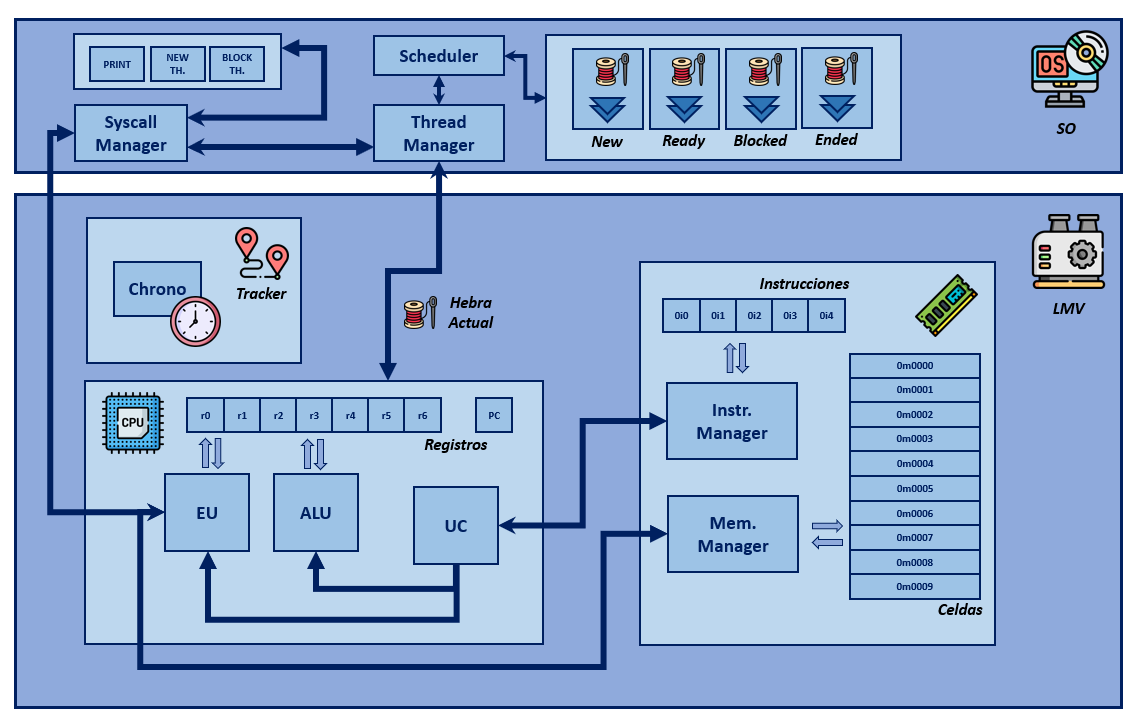
\includegraphics[width=\linewidth]{images/lmp/LVM_resume.png}
    \caption{Esquemático de la Máquina Virtual de Lamport}
    \label{fig:LVMResume}
\end{figure}

\begin{itemize}
    \item \textbf{CPU (~\ref{subsubsec:CPULVM} )}: El núcleo de procesamiento, que realiza operaciones aritméticas, lógicas y de control. Incluye un conjunto de registros, un contador de programa y una Unidad de Ejecución.
    
    \item \textbf{Memoria (~\ref{subsec:memoryLVM} )}: Almacena datos e instrucciones, optimizando el acceso y gestión de la información.

    \item \textbf{Sistema Operativo (~\ref{subsec:SOLVM} )}: Administra recursos y facilita la interacción entre software y hardware simulado.
\end{itemize}

\subsection{CPU}\label{subsubsec:CPULVM}
La CPU es responsable de ejecutar instrucciones y gestionar operaciones. Incluye un vector de registros para almacenamiento temporal, un contador de programa para seguimiento de instrucciones, una Unidad Aritmético Lógica (ALU) para operaciones matemáticas y lógicas, una Unidad de Control para coordinar actividades, y una Unidad de Ejecución para llevar a cabo instrucciones.

\subsubsection{Registros}\label{subsubsec:registrosLVM}
Los registros son de las partes más importantes de la CPU en la máquina virtual, ya que albergan y gestionan los valores que las instrucciones de operación requieren para su ejecución, principalmente para tareas de consulta y modificación. Siguiendo el esquema de registros "infinitos" discutido en ~\ref{subsec:asignacionRegIR}, la estructura del vector de registros se organiza de la siguiente manera:
\begin{itemize}
    \item \textbf{Registros r0 - r30}: Registros dedicados a parámetros y variables locales de subprogramas.
    \item \textbf{Registro r31}: Registro dedicado al retorno de una función.
    \item \textbf{Registros r32 en adelante}: Registros de propósito general.
\end{itemize}

\subsection{Esquema de ejecución de código en LVM}
Finalmente, lo que queda es comentar cómo es el esquema general de ejecución de instrucciones IR en la Máquina Virtual de Lamport:

\begin{enumerate}
    \item Creación de la tabla de segmentos y volcado de contenidos iniciales en la memoria.
    \item Iniciación de hebras correspondientes a procesos estáticos y una hebra maestra encargada de comenzar la ejecución.
    \item Decisión de qué hebra ejecuta el procesador en cada ciclo de CPU mediante un planificador.
    \item Finalización del programa cuando se alcanza \code{IR_END_PROGRAM} o todos los procesos terminan su ejecución.
\end{enumerate}

\subsection{Memoria}\label{subsec:memoryLVM}
La memoria de la LVM utiliza un mapa ordenado para simular una memoria física. Se gestiona mediante un esquema segmentado para organizar diferentes tipos de datos y facilitar la traducción de direcciones virtuales a físicas.

\subsubsection{Tabla de segmentos}\label{subsubsec:pageTableLVM}
La tabla de segmentos administra la correspondencia entre direcciones lógicas y físicas, organizando segmentos para literales, etiquetas, variables globales, índices y variables locales de procesos.


A continuación se especifican los segmentos definidos y los rangos de direcciones físicas asignados:

\begin{itemize}
    \item \textbf{Segmento 0 (literales):} Desde la dirección 0 hasta la dirección 999.
    \item \textbf{Segmento 1 (etiquetas):} Desde la dirección 1000 hasta la dirección 1999.
    \item \textbf{Segmento 2 en adelante (variable):} Desde la dirección 2000 en adelante. Aquí se definen múltiples segmentos consecutivos dependiendo de:
    \begin{itemize}
        \item Si hay variables globales (segmento 2).
        \item Si hay índices de bucles (segmento 3).
        \item Número de procesos (segmento 4 en adelante).
    \end{itemize}
\end{itemize}

\subsubsection{Iniciador de la memoria}
En la fase de generación de código intermedio, específicamente en la tabla de variables, hay un campo denominado \textit{valor inicial}. Simplemente contiene el valor de inicio de la variable en función del tipo de dato, por ejemplo 0 para los enteros, o la cadena vacía para los strings. Teniendo en cuenta esto y el esquema de segmentación implementado anteriormente, se decidió desarrollar una clase encargada de volcar a memoria todo el contenido de todas las tablas en los bloques de memoria correspondientes a las direcciones físicas.

\subsection{Sistema Operativo}\label{subsec:SOLVM}
El sistema operativo de la LVM gestiona la interacción entre software y hardware simulado. Sus responsabilidades incluyen el manejo de llamadas al sistema, coordinación de la CPU con el planificador de procesos, y gestión de bloqueo y terminación de procesos.

\subsection{Estado de la memoria de LVM con ``HolaMundo''}
Se acerca el momento en el que el programa ``HolaMundo'' (~\ref{fig:lamportHolaMundo} ) podrá ser ejecutado como un lenguaje cualquiera, pero antes de ello se muestra la fase donde el contenido de las tablas de literales, variables y etiquetas definidas en ~\ref{fig:IRHolaMundo} se vuelca a la memoria de la máquina.


\noindent
Este es el resultado de la ejecución del iniciador de memoria:
\begin{verbatim}
==========================================================
TABLA DE SEGMENTOS
==========================================================
Segmento número (0) : literales
==========================================================
Dirección Virtual    Dirección Física    
==========================================================
0                     0m00000000            
1                     0m00000001            
2                     0m00000002            
3                     0m00000003            
4                     0m00000004            
5                     0m00000005            
6                     0m00000006            
==========================================================

Segmento número (1) : etiquetas
==========================================================
Dirección Virtual    Dirección Física    
==========================================================
0                     0m00001000            
1                     0m00001001            
2                     0m00001002            
3                     0m00001003            
4                     0m00001004            
5                     0m00001005            
6                     0m00001006            
==========================================================

Segmento número (2) : variables globales
==========================================================
Dirección Virtual    Dirección Física    
==========================================================
0                     0m00002000            
==========================================================

Segmento número (3) : indices
==========================================================
Dirección Virtual    Dirección Física    
==========================================================
==========================================================

Segmento número (4) : Main
==========================================================
Dirección Virtual    Dirección Física    
==========================================================
4                     0m00002001            
5                     0m00002002            
==========================================================

==========================================================
MEMORIA DE LA MÁQUINA VIRTUAL
==========================================================
Dirección            Tipo de bloque        Contenido             
==========================================================
0m00000000            string                "Hola ""             
0m00000001            string                "!"                 
0m00000002            integer               0                     
0m00000003            integer               18                    
0m00000004            string                "Daniel"            
0m00000005            integer               23                    
0m00000006            string                "El numero magico vale: "
0m00001000            instr. address        0i0001                
0m00001001            instr. address        0i0004                
0m00001002            instr. address        0i0013                
0m00001003            instr. address        0i0014                
0m00001004            instr. address        0i0022                
0m00001005            instr. address        0i0025                
0m00001006            instr. address        0i0042                
0m00002000            integer               0                     
0m00002001            string                ""                    
0m00002002            integer               0                     
\end{verbatim}
\begin{figure}[hbtp]
\caption{Programa ``¡Hola Mundo!'' Lamport: Tabla de segmentos y memoria de LVM en su estado inicial.}
\label{fig:preLVMHolaMundo}
\end{figure}

\subsection{Control de excepciones}
Como se mencionó en ~\ref{subsec:semanticaLamport}, el lenguaje Lamport es \textit{inseguro}. Esto pone en manos del programador la responsabilidad de garantizar la corrección de ciertas operaciones. Sin las debidas precauciones, el comportamiento del programa podría ser indeterminado. Esta circunstancia destaca la necesidad de implementar un mecanismo de \textit{excepciones}.


Una excepción juega un papel crucial en la gestión de errores y situaciones inesperadas durante la ejecución de un programa. Sirve como mecanismo de señalización que indica que algo ha ido mal o que ha surgido una condición no prevista.


\noindent
La Máquina Virtual de Lamport es capaz de tratar dos tipos de excepciones:
\begin{itemize}
    \item \textbf{Excepción ZeroDivision:} Se produce cuando se intenta realizar una operación de división, cuyo segundo operando (divisor) es el número 0.
    \item \textbf{Excepción OutOfBounds:} Se produce cuando se intenta relizar un acceso indebido a un array, esto es, una posición fuera de los límites que le corresponden.
\end{itemize}

\section{Hebras y planificación}
Dado que el motivo principal de este proyecto es \textit{simular concurrencia}, se ha considerado pertinente dedicar este espacio específico para tratar en profundidad la implementación y gestión de hebras, así como el mecanismo de planificación que las coordina. A continuación, se detallan los mecanismos y estrategias adoptadas para lograr una simulación fiel y eficiente de la concurrencia en la Máquina Virtual.

\subsection{Tipos de hebras}
En la Máquina Virtual hay diferentes tipos de hebras dependiendo de su naturaleza, enumerándose a continuación:

\begin{itemize}
    \item \textbf{Iniciadora}. Es una hebra especial que se crea una única vez, al inicio del programa. Su misión es inicializar las variables globales si las hay. Acto seguido, se destruye y se empieza el ciclo de CPU con las hebras de proceso.
    \item \textbf{Estáticas}. Estas hebras son aquellas que corresponden a un proceso de Lamport y están definidas desde el inicio del programa. Su existencia y características se determinan en tiempo de traducción, y no varían durante la ejecución del programa.
    \item \textbf{Dinámicas:} Son hebras creadas en tiempo de ejecución, dependiendo del flujo y las condiciones del programa. Un claro ejemplo de la creación de una hebra dinámica es cuando se ejecuta una instrucción del tipo \code{fork}. Estas hebras ofrecen una gran flexibilidad, adaptándose a las necesidades y circunstancias que surgen durante la ejecución del programa.
\end{itemize}

\subsection{Implementación de hebras}
Cada hebra en la LVM es una unidad mínima de ejecución y se compone de varios elementos como identificador, estado, segmento de memoria, registros, pila de ejecución, contador de instrucciones, quantum, y en el caso de hebras hijas, una referencia al proceso padre.

\subsection{El modelo de 5 estados para Hebras}

El modelo de 5 estados representa un marco conceptual que permite entender y categorizar las diferentes etapas o fases por las que una hebra puede pasar durante su ciclo de vida. Cada estado ofrece una perspectiva única sobre la condición y actividad de la hebra. A continuación, se describen brevemente estos cinco estados:

\begin{enumerate}
    \item \textbf{Nuevo (New):} En este estado, la hebra ha sido creada pero aún no ha comenzado su ejecución. Está esperando la asignación de recursos necesarios para iniciar.

    \item \textbf{Listo (Ready):} La hebra está lista para ejecutarse y está esperando ser asignada a un procesador por el planificador. Todos los recursos necesarios ya han sido asignados, pero la hebra no está siendo ejecutada en este momento.

    \item \textbf{En ejecución (Running):} La hebra ha sido asignada a un procesador y está siendo ejecutada actualmente. En este estado, la hebra realiza sus tareas designadas.

    \item \textbf{Bloqueado (Blocked):} Aquí, la hebra está esperando un evento o recurso específico para continuar. Puede estar esperando la conclusión de una operación de I/O, la liberación de un recurso, o cualquier otro evento que impida su ejecución continua.

    \item \textbf{Terminado (Terminated):} La hebra ha completado su ejecución y ha finalizado todas sus tareas. Una vez que una hebra alcanza este estado, no puede regresar a los estados anteriores.
\end{enumerate}

Este modelo proporciona una estructura clara para visualizar y entender el flujo y transiciones que una hebra experimenta, facilitando la gestión y control de la concurrencia en sistemas informáticos.

\begin{figure}[h]
    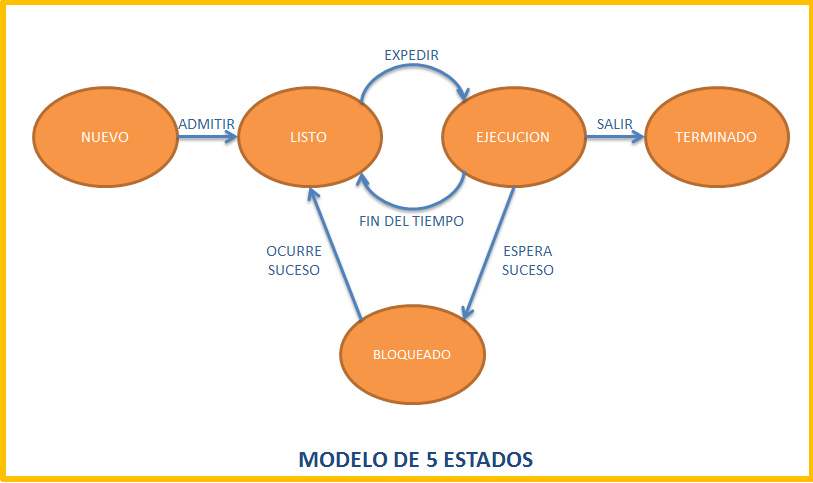
\includegraphics[width=\linewidth]{images/implementacion/hebras/modelo5_estados.png}
    \caption{Modelo de 5 estados para hebras. Diagrama de transiciones.}
    \label{fig:modelo_estados_hebras}
\end{figure}

\newpage

\subsection{Planificador. Esquema Round-Robin con Quantums aleatorios}
El esquema de planificación Round-Robin con Quantums aleatorios de la LVM introduce una variabilidad en el tiempo de ejecución asignado a cada hebra, añadiendo un factor dinámico para mejorar la eficiencia del sistema.

A continuación se explica el concepto de \textbf{quantum aleatorio}: cada hebra recibe un \textit{quantum}, definido como el número de instrucciones permitidas para ejecutar antes de ceder el CPU, que varía aleatoriamente entre 1 y 4 instrucciones. Este enfoque busca optimizar la asignación de recursos ajustándose a las condiciones del sistema.

\subsubsection{Componentes del planificador}
\noindent
El planificador, además de su algoritmo de planificación, consta de los siguientes elementos:
\begin{itemize}
    \item Una cola de hebras nuevas.
    \item Una cola de hebras listas.
    \item Una cola de hebras bloqueadas.
    \item Una cola de hebras terminadas.
    \item Un puntero a la hebra que está actualmente ejecutando.
\end{itemize}

\subsubsection{Proceso de planificación}
Finalmente, se describe el esquema de planificación Round-Robin definido para la simulación de la concurrencia entre hebras:
\begin{enumerate}
    \item \textbf{Inicialización}: Todas las hebras nuevas se mueven a la cola de listas y se elige una al azar para empezar la ejecución.
    \item \textbf{Ejecución Continua}: Si solo hay una hebra activa, controla el CPU indefinidamente.

    \item \textbf{Selección de Hebras}:
    \begin{enumerate}
        \item Si hay, se añaden hebras nuevas a la cola de listas.
        \item Si una hebra termina, se mueve a la cola de terminadas y notifica a su hebra padre si es aplicable.
        \item Si una hebra excede su quantum, se reubica al final de la cola de listas y se selecciona la siguiente hebra para ejecución. En caso contrari, si todavía dispone de tiempo en CPU, sigue controlándola.
    \end{enumerate}

\end{enumerate}

Este esquema garantiza un balance entre equidad y eficiencia, permitiendo a las hebras compartir el CPU de manera justa y adaptativa, además de realizar una simulación más realista.

\section{Gestión de señales de interrupción UNIX (POSIX)}\label{sec:posixSignalsLMP}
En el desarrollo de la Máquina Virtual de Lamport, se ha implementado un mecanismo de gestión de señales de interrupción UNIX, siguiendo el estándar POSIX, con especial atención a la señal de interrupción Ctrl+C (SIGINT). Este mecanismo desempeña un papel crucial en la operación segura y controlada de la máquina virtual, especialmente en situaciones de bloqueo o ejecución de bucles infinitos.

La interrupción Ctrl+C es una señal común en los entornos de sistemas operativos UNIX para solicitar la terminación de un proceso en ejecución. En el contexto de la Máquina Virtual de Lamport, esta señal ha sido configurada para funcionar como un mecanismo de detención segura. Al detectar la señal de interrupción, la máquina virtual inicia un proceso de cierre ordenado, asegurando que todos los recursos y procesos en ejecución se gestionen adecuadamente antes de la terminación.

La implementación de este mecanismo de gestión de señales no solo mejora la robustez de la Máquina Virtual de Lamport, sino que también enriquece la experiencia del usuario al proporcionar una forma efectiva y segura de manejar situaciones inesperadas durante la ejecución del programa. Además, alinea la máquina virtual con las prácticas estándar en entornos UNIX, facilitando su integración y uso en estos sistemas.

\section{Interfaces de control de intérprete: ``LMP Utils``}\label{sec:implementacionLMPUtils}
Hasta ahora se han definido y desarrollado una gran cantidad de módulos que se comunican entre sí de varias formas. Es por ello por lo que es necesario establecer una vía de control de forma sencilla y unificada entre cada módulo y la función principal del intérprete que es quien ejecuta todos los analizadores y clases en el orden que corresponde. En total se han definido un total de 5 controladores diferentes:

\begin{itemize}
    \item \textbf{Controlador de flujos de E/S:} Es el encargado de realizar el tratamiento de apertura y cierre del fichero de código Lamport a ejecutar.
    \item \textbf{Controlador de Análisis:} Es el encargado de ejecutar los analizadores sintáctico y semántico, y de mantener el AST del programa, enviando al intérprete los errores en caso de que se produzcan.
    \item \textbf{Controlador de IR:} Es el encargado de llamar al optimizadador de AST y constructor de instrucciones de código intermedio.
    \item \textbf{Controlador de LVM:} Es el encargado de lanzar la máquina virtual cuando se ha generado el código intermedio.
    \item \textbf{Controlador de registros de eventos (logging):} Este controlador es especial y extremadamente útil para el usuario del intérprete. Su función es registrar todos los eventos que se han producido en el intérprete, desde el análisis sintáctico pasando a la generación de código intermedio, estado de la memoria de la LVM y traza de ejecución, o la generación de errores.

    Genera un directorio denominado \code{log/} que contiene los ficheros de logging siguientes:
    \begin{itemize}
        \item \textbf{logging de AST}: Contiene el AST generado para el programa.
        \item \textbf{logging de IR}: Contiene las tablas de literales, variables y etiquetas, y el listado de instrucciones IR.
        \item \textbf{logging de LVM}: Contiene la tabla de segmentos y el estado de la memoria en el inicio de la máquina lamport, además de la traza de ejecución de la máquina al terminar. Además, también genera un fichero de registro con toda la traza de ejecución del programa en la Máquina Virtual.
        \item \textbf{logging de errores}: Contiene el listado de errores producidos en el análisis.
    \end{itemize}
\end{itemize}

\section{Ejecución de ``HolaMundo''}
Se ha llegado al final del proyecto, donde por fin se puede ejecutar el programa ``HolaMundo'' (~\ref{fig:lamportHolaMundo} ) del que tantas veces se ha hablado a lo largo de estas secciones. 


\noindent
El resultado de la ejecución es el siguiente:
\begin{figure}[h]
  \begin{minipage}{\linewidth}
    \centering
    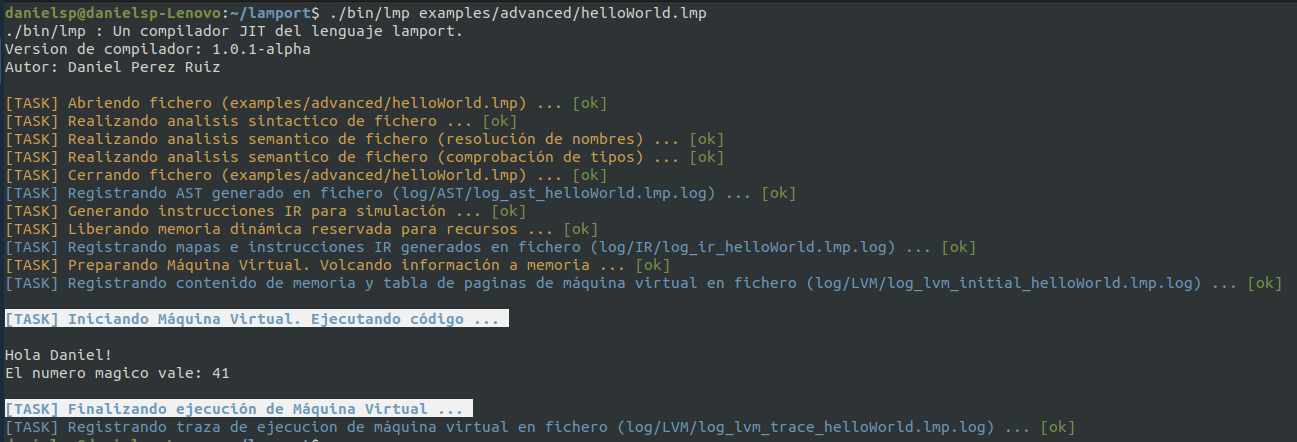
\includegraphics[width=\linewidth]{images/implementacion/ejecucion/lmp_hola_mundo.png}
    \caption{Ejecución de ``HolaMundo'' en el intérprete.}
    \label{fig:ejecucionHolaMundo}
  \end{minipage}
  \vspace{10pt} 
  \begin{minipage}{\linewidth}
    \centering
    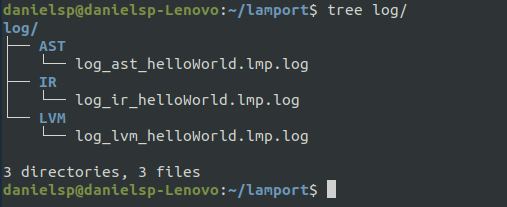
\includegraphics[width=\linewidth]{images/implementacion/ejecucion/logs.png}
    \caption{Ficheros de logging generados tras la ejecución.}
    \label{fig:logsHolaMundo}
  \end{minipage}
\end{figure}

\newpage
\subsection{Traza de ejecución de ``HolaMundo''}
Al finalizar la máquina virtual, se genera un fichero de registro con todas las operaciones que ésta ha ido realizando a nivel de CPU y de memoria. En la siguiente imagen se muestra la cabecera de la traza de ejecución para el programa ``HolaMundo'':
\begin{figure}[h]
  \begin{minipage}{\linewidth}
    \centering
    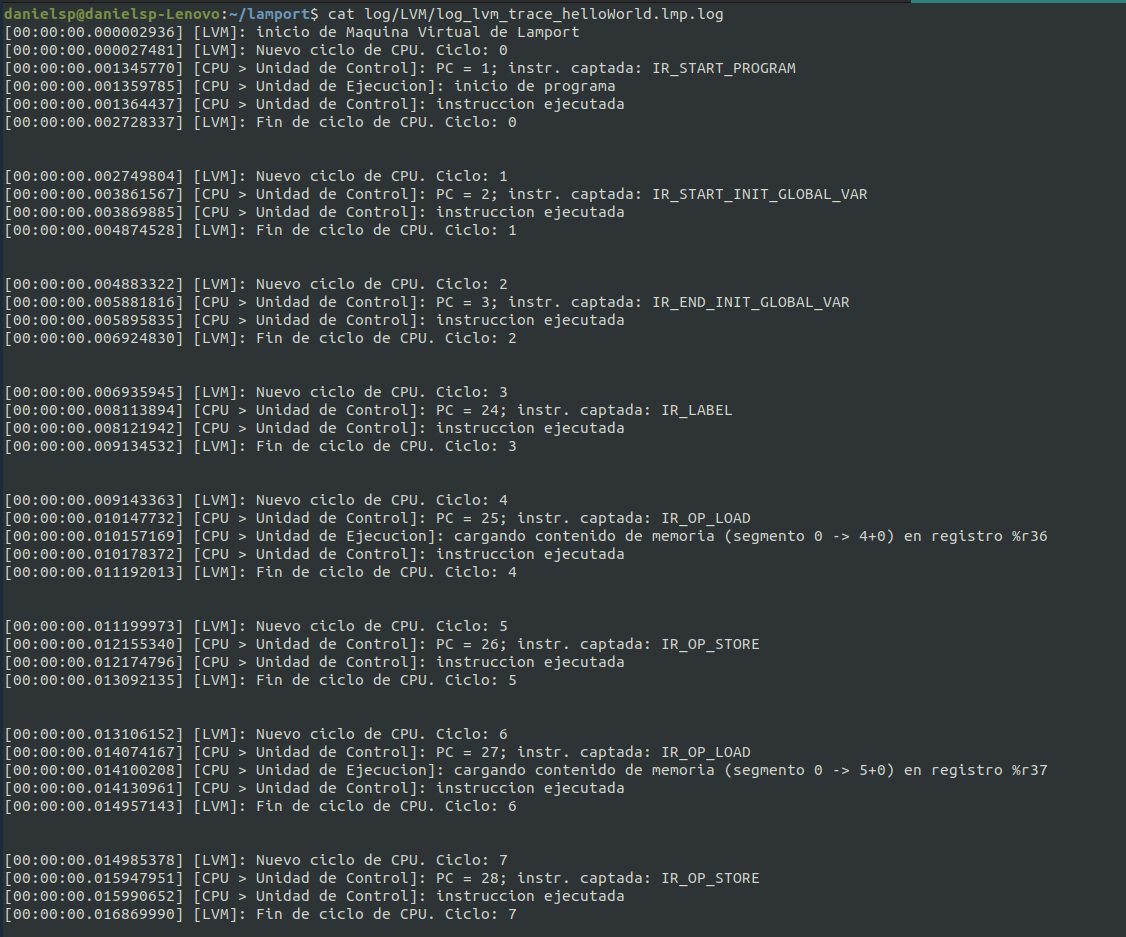
\includegraphics[width=\linewidth]{images/implementacion/ejecucion/resumed_traza.png}
    \caption{Traza de ejecución de ``HolaMundo''.}
    \label{fig:trazaHolaMundo}
  \end{minipage}
\end{figure}

\newpage
\section{Dockerización del intérprete}
Con la evolución constante de la tecnología y las infraestructuras de software, la necesidad de crear aplicaciones portables y escalables ha cobrado mayor importancia. Docker, una herramienta que permite la creación de contenedores, surge como una solución a esta demanda. Un contenedor Docker encapsula una aplicación junto con todas sus dependencias en una unidad estándar de software, garantizando que la aplicación se ejecute de la misma manera sin importar dónde se despliegue. 



En el contexto del intérprete desarrollado, la dockerización ofrece ventajas significativas en términos de portabilidad, aislamiento y replicabilidad. Esta sección detallará el proceso y las consideraciones adoptadas al dockerizar el intérprete, permitiendo su distribución y ejecución de manera homogénea en diferentes entornos.

\subsection{Construcción del contenedor}
Para construir el contenedor Docker que encapsulará el intérprete junto con todas sus dependencias, se han realizado las siguientes tareas:

\begin{enumerate}
    \item Elección de una imagen base. Ésta debe ser del menor tamaño posible para que sólo contenga lo imprescindible, además de ser una imagen que reciba constantes actualizaciones de seguridad y mantenimiento. En el caso de este proyecto, \textbf{alpine} es una excelente elección por cumplir estas dos características.
    \item Construir el fichero \code{Dockerfile}. Este fichero indica cómo se debe construir el contenedor de forma automática, aprovisionándolo de todas las dependencias.
    \item Definir script de ejecución utilizando el contenedor virtual. Para hacer aún más fácil el uso de esta herramienta se definió un script denominado \code{./lmp_docker.sh} que ejecuta el contenedor utilizando como argumento el fichero de código Lamport indicado.
\end{enumerate}

\subsection{Compilación estática del intérprete}
La compilación estática se refiere al proceso de integrar todas las bibliotecas y dependencias requeridas por una aplicación directamente en el binario ejecutable, en lugar de depender de bibliotecas compartidas en el sistema en tiempo de ejecución. Este método tiene varias ventajas, especialmente en el contexto que concierne a esta sección:

\begin{itemize}
\item \textbf{Portabilidad mejorada}: Un binario estáticamente enlazado no tiene dependencias externas, lo que garantiza que funcionará en cualquier entorno que lo ejecute, eliminando así problemas relacionados con versiones de bibliotecas o dependencias faltantes.
\item \textbf{Reducción del tamaño del contenedor}: Al no requerir la instalación de bibliotecas adicionales en el contenedor (sólo se necesita instalar flex y bison de manera inevitable), el tamaño de la imagen resultante puede reducirse significativamente. En este proyecto, la imagen del contenedor se redujo de 249 MB a tan solo 24 MB, una optimización impresionante.
\item \textbf{Seguridad mejorada}: Al reducir el número de componentes en el contenedor, se disminuye la superficie de ataque potencial, al eliminar software adicional que no es esencial para la aplicación pero que podría presentar vulnerabilidades.
\end{itemize}

Para lograr la compilación estática del intérprete, se utilizaron las herramientas gcc y g++ con las opciones de enlazado estático. Además, se aprovechó el enfoque de construcción multi-etapa en Docker, donde la primera etapa incluye todas las herramientas y dependencias necesarias para la compilación, y la segunda etapa simplemente copia el binario resultante, resultando en una imagen Docker final limpia y optimizada.

\begin{figure}[h]
    \begin{adjustbox}{center}
        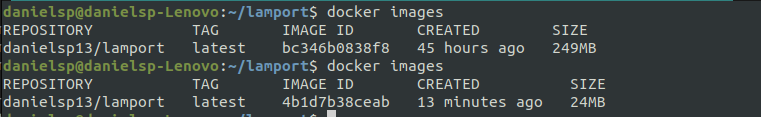
\includegraphics[width=\linewidth]{images/implementacion/docker/docker_reduce.png}
    \end{adjustbox}
    \caption{Tamaño de contenedor docker antes y después de usar compilación estática.}
    \label{fig:DockerReduce}
\end{figure}